\documentclass[UKenglish]{book}
\setcounter{tocdepth}{4}
\setcounter{secnumdepth}{4}
\newcommand\hmmax{0}
\newcommand\bmmax{0}

\counterwithout{footnote}{chapter}
\usepackage{Setup/style}
\DeclareMathAlphabet{\mathcal}{OMS}{cmsy}{m}{n}
\raggedbottom %%reduces the gaps between the paragraphs
\usepackage{jheppub}

\title{Bayesian Neural Network Estimation of Next-To-Leading-Order Cross Sections}
%\subtitle{My subtitle}
\subsubtitle{by}
\author{René Alexander Ask}
\thesistext{THESIS}
\thesistextt{for the degree of}
\thesistexttt{MASTER OF SCIENCE}


\bibliographystyle{JHEP}
%\addbibresource{bibliography.bib}
%\DeclareUnicodeCharacter{2212}{-}
%\DeclareUnicodeCharacter{03B1}{-}

\begin{document}
\duoforside[dept={Department of Physics},
  program={Master's Program Name},
  long]
%%%%%%%%%%%%%%%%%%%%%%%%%%%%%%%%%%%%%%%%%%%

\frontmatter{}
\chapter*{Abstract} 
Near the kinematical production threshold scattering cross sections gain large logarithmic corrections. This is due to the fact that close to the threshold the radiation of gauge bosons is restricted to be soft. This leads to an imbalance in the cancelling between real and virtual contributions at higher order, leading to large logarithmic contributions. In order to make reliable predictions such contributions must be resummed. In this thesis we make use of an object called a Wilson line to describe the soft radiation. Wilson lines are path-ordered exponentials of the gauge fields. They contain all the kinematical and dynamical information from the gauge sector and are central in taking a geometrical viewpoint of quantum field theory, and in particular quantum chromodynamics. We mainly consider semi-infinite Wilson lines on linear paths, which naturally describes radiation from highly energetic particles. By constructing a special class of Wilson lines, namely Wilson lines on closed paths called Wilson loops, we show how the soft radiation can be fully characterized by a so-called eikonal cross section. From an explicit one-loop calculation of a Wilson loop expectation value we find the universal cusp anomalous dimension. This cusp anomalous dimension is shown to be a central ingredient in evolution equations for Wilson lines, perturbative distributions and subsequently for eikonal cross sections. With the aid of the cusp anomalous dimension we find an exponentiated form of the Drell-Yan cross section up to leading logarithmic order. 
\chapter*{Acknowledgements}
First of all, I want to thank my supervisor, Are Raklev, for practical advice on my master's thesis. The contextual explanations of the underlying physics and its pertinent challenges have provided me with precisely the amount of knowledge necessary to carry out the work in this thesis. I have enjoyed your calm nature and acceptance of my pragmatic approach to writing. I also want to thank Anders Kvellestad for serving as my unofficial co-advisor. You have taken time to have lengthy discussions of possible theoretical approaches and you have given me valuable insights into certain aspects of computing and interpretation of Bayesian statisics. 

I will never forget the friends I gained through my studies. I want to thank you all for enhancing my experience and helped me grow as a human. It has been a pleasure to learn about the inner-workings of Mother Nature beside you. It was the best of times, it was the worst of times. A special thanks to Toshi for awesome long nights working through our bachelor's courseload and long walks after late nights out, to Bennern for emotional support and wisdom to carry out life-changing decisions, to Maria for your friendship and the christmas celebration I got to spend with your family, to Kaspara for your inability to stop talking and being the life-of-the-party, to Une for being the best labpartner I could ever get and unexpectedly arranging a celebration for my birthday last year, to my boy TK for being my ``homie'' for more than 20 years, to Isak and Karianne for your unfiltered speech and so many more. Rest assured, besides a couple examinators, no one will read this thesis. Thus if your name is omitted, no one will ever know.

A final thanks to the Norwegian government for allowing me the opportunity to pursue an education of high quality at no cost and for the computing resources used in this thesis. Now that we are mentioning education, thanks to every single person that has dedicated their life to understanding nature and progressing our collective base of knowledge. Without them, there would be no education to speak of. 

\tableofcontents{}
\listoffigures
\listoftables
\listofalgorithms

%%%%%%%%%%%%%%%%%%%%%%%%%%%%%%%%%%%%%%%%%%%
\mainmatter{}
\chapter*{Introduction}
\addcontentsline{toc}{chapter}{Introduction}


The Standard Model of particle physics is a remarkably successful theory explaining the fundamental particles of nature and their interactions. It accounts for the constituent building blocks of all everyday phenomena on Earth. Yet, there exist a vast number of observations gathered in collider experiments which the Standard Model cannot account for. 
This has led physicists to propose several extensions to the theory.
These extensions, collectively called Beyond the Standard Model theories, predict the existence of new phenomena that may explain the observed data. The investigation of the extended theories needs a high accuracy in its computed predictions. Direct calculation of these demands an excessive computational cost which significantly hampers the search for new physics. The use of machine learning to 
circumvent this obstacle has steadily increased over the last years with hopes of speeding up the search. The use of modern machine learning models such as deep learning has been widely used for classification tasks but the use of machine learning models to perform regression tasks in high-energy physics has only recently been employed to speed up quantum field theory calculations that would otherwise be intractible by direct calculation. An example of this effort is through evaluation of higher-order cross sections using Gaussian processes \cite{xsec}. 

Classical regression is insufficent, however. A crucial aspect of regression tasks in high-energy physics is an estimation of the uncertainty in predictions which are needed to properly evaluate a new physics model by propagation of the uncertainty through proper inference models. While deep neural networks are ubiquitously employed to solve regression problems in the real world, they suffer the need for an excessive amount of data to serve as robust and reliable tools for predicting unknowns, which can be a major drawback of the model class for smaller sets of data. However, neural networks are universal function approximators and serve as an ideal model class for regression tasks, especially in the case where the underlying relationship one attempts to regress is difficult to discern from first principles. Bayesian inference of its parameters offers an approach of obtaining a distribution of its parameters which allow for computation of predictions and yield corresponding uncertainty estimates. The most widely used method for inferring parameters of neural networks through the Bayesian framework is to parameterize a surrogate distribution for its weights which are used to approximate its true distribution. The approach has spawned a popular research area because of its natural integration into popular machine learning frameworks such as TensorFlow and PyTorch with the goal of spending approximately the same amount of time adjusting its parameters as it does for classical neural networks. The potential weakness is of course its approximation of the exact distribution of weights. 

In this thesis, we propose using Hamiltonian Monte Carlo and its derivatives to infer neural network parameters from its exact distribution. It is a class of Markov chain Monte Carlo (MCMC) methods for continuous sample spaces. It is well known to be computationally expensive for large datasets but in the search for physics beyond the Standard Model, data is a scarce resource, a scenario in which a more accurate approach to inference may shine. Bayesian inference using Hamiltonian Monte Carlo to sample from the exact distribution is considered challenging at best, as neural networks suffer from unidentifiability. The model class is what is known as over-parameterized. This gives rise to multiple equivalent parameterizations that all yield the same predictions which has the unfortunate consequence of potentially producing multi-modal distributions with many regions that all yield the same effective predictions. Although Hamiltonian Monte Carlo is considered a state-of-the-art sampling method for continuous sample spaces, it needs hand-tuning to achieve good results. To handle this, we will explore adaptive Hamiltonian Monte Carlo methods to automatically perform tuning on the fly.

The main objective of this thesis is to investigate the viablity of substituting direct calculation of next-to-leading order cross sections in quantum field theory with Bayesian neural networks drawn from its exact distribution of parameters.
To this end, we will investigate the computational cost of the inference using Hamiltonian Monte Carlo and adaptive extensions of it. A central point of interest is the actual time needed to infer parameters on modern computing hardware like CPUs and GPUs to evaluate the feasibility of the methods. The computational cost of computing predictions of inferred models is a related and equally important question which we will consider. The distribution of neural network parameters are reported to be multi-modal \cite{google_bnn_posteriors}, a feature we will investigate. Due to the need for reliable uncertainty estimates when predictions are fed through proper inference models, we will investigate the predictive performance of Bayesian neural networks and the quality of the uncertainty estimates they yield. Inference of neural network parameters require the specification of a large number of hyperparameters, the effect of which may be highly dependent on the underlying data used. We will therefore investigate the effect these have on computational cost and predictive performance.

\subsubsection*{Outline of the Thesis}
In chapter \ref{chap:physics_problem}, we will discuss the extensive computational cost needed to compute next-to-leading order cross sections in quantum field theory and how Bayesian regression models can serve as a viable substitute for direct calculation of these. 
In chapter \ref{chap:bayesian_ml}, we will give an overview of machine learning for regression tasks and a formulation of it from a Bayesian perspective. We will discuss how one in general constructs a probabilistic model using Bayes' theorem which all together culminates to the notion of Bayesian machine learning.
In chapter \ref{chap:mcmc}, we provide an overview of important ideas for Monte Carlo Markov chains in continuous sample spaces including the Metropolis-Hastings and Gibbs samplers which form the basis for Hamiltonian Monte Carlo. In chapter \ref{chap:hmc} we will present Hamiltonian dynamics and discuss how we can construct the basic Hamiltonian Monte Carlo sampler. 
In chapter \ref{chap:no_u_turn_sampler} we explore ways to dynamically tune parameters used in the sampler to avoid tedious hand-tuning and automatically tune them on the fly. In chapter \ref{chap:bnn}, we will survey the neural network model before we bring all the topics together, culminating in a training algorithm for Bayesian neural networks using the MCMC samplers to draw parameters directly from the exact distribution of the model. In chapter \ref{chap:methodology}, we will discuss the dataset we apply the methods to, the preparation of the data and present the metrics we will use to evaluate the performance of the inferred models. In chapter \ref{chap:numerical_experiments}, we will present the results of our numerical experiments and discuss their implications. In chapter \ref{chap:conclusion}, we will present our final thoughts on the methods and suggestions for future topics of investigation.


\begin{comment}
    The two most common classes are weight-space symmetry and scaling symmetry. The first symmetry refers to the case where two layers can be permuted and still produce the same prediction. The second symmetry arise when using non-linear function that obey $\sigma(\alpha x) = \alpha\sigma(x)$. The second symmetry can be removed entirely by avoidance of non-linear function of this form but the first symmetry is an unavoidable one. Thus many equivalent parameterizations exist which manifest itself as a multi-modal distribution that can be notoriously difficult to infer parameters from.
\end{comment}
	
%%%%%%%%%%%% Neural networks %%%%%%%%%%%%%%
%\chapter{Methods}\label{chap:methods}
\chapter{The Physics Problem}
In this chapter, we shall motivate the need for Bayesian machine learning regression models to replace deterministic methods in high-energy physics in the search for Beyond the Standard Model (BSM) physics. We will start off with a brief survey of the conventional way to compute cross sections, its need for precision and the inherent problems involved. We will end the chapter with a discussion of how Bayesian regression can provide a substitute for the standard way to compute cross sections.


\section{Computation of Beyond the Standard Model Cross Sections}
The Standard Model of particle physics (SM) is a successful fundamental theory that describes the fundamental particles of nature and their interactions.  Despite its success, however, it has a few limitations on its own which has led physicists to propose extentions to the model to explain physics that the SM cannot. One such family of extensions is called \textit{supersymmetry}. Theories like this are known as BSM models. 

In order to test whether a particular symmersymmetric extension to the SM is valid, one has to search through large (high-dimensinoal) parameter spaces where the parameters themselves somewhat simplified represent the properties of the particles in the model. The technical aspect is to rather \textit{exclude} regions of parameter space which cannot explain observed data. To this end, theoretical physicists must compute what is known as a \text{cross section} $\sigma$. These are roughly speaking the probability that a particular \text{event} occurs in a particular collider experiment. The total number of such events is given by the \textit{event equation}
\begin{equation}\label{eq:event_equation}
    n = \sigma \epsilon A \mathcal{L},
\end{equation}
where $\epsilon$ represents the efficiency of the experimental apparatus, $A$ represents the acceptance and $\mathcal{L}$ is the integrated luminosity of the data taken in the search or experiment, i.e. the amount of data. The job of the theoretical physicist is to compute $\sigma$, as all the other quantities can be inferred or measured from the experimental setup used.

We may further decompose the total number events as
\begin{equation}\label{eq:total_events_decomp}
    n = s + b,
\end{equation}
where $b$ is called the \textit{background} which is the portion of the events explained by the SM. Here $s$ represents a portion of $n$ which cannot be explained by SM, but rather the new BSM model, and is called the \textit{signal}. Strictly speaking, the model proposed may only explain a subset of the total events. 
On a more technical level, the event equation can be divided into several \textit{cuts}. A cut defined a range of an experimentally measured quantity where anything outside of it is excluded. A \textit{signal region} consists of a set of cuts. For a signal region $i$, the event equation reads
\begin{equation}\label{eq:general_event_eq}
    n_i = \sigma \epsilon_i A_i \mathcal{L}.
\end{equation} 
All but the cross section and the integrated luminosity depend on the signal region.

The computation of $\sigma$ in eq.~\eqref{eq:event_equation} needs to be carried out to a high accuracy to yield a greater exlusion power. To explain why, consider the Poisson likelihood
\begin{equation}\label{eq:poisson_likelihood}
    \mathcal{L}(n|s, b) = \int_0^\infty \frac{[\xi(s + b)]^n e^{-\xi(b + s)}}{n!}P(\xi)\dd \xi,
\end{equation}
where $\xi$ is a rescaling parameter and $P(\xi)$ is its probability distribution which is peaked at $\xi = 1$.
Its width is defined by
\begin{equation}\label{eq:xi_width}
    \sigma_\xi^2 = \frac{\sigma_s^2 + \sigma_b^2}{(s + b)^2},
\end{equation}
where $\sigma_s$ is the systematic uncertainty of the signal predictions $s$ and $\sigma_b$ is the systematic uncertainty of the background $b$. The particular form of $P(\xi)$ given a width $\sigma_\xi$ is typically chosen to be Gaussian or log-normal \cite{colliderbit}.
To compare $s$ and $b$ correctly to $n$ we must evaluate eq.~\eqref{eq:poisson_likelihood}. If $\sigma_s$ is large, this will increase the width $\sigma_\xi$ which yields a larger value of the likelihood for all points $\xi$. The consequence is less exclusion power achieved by the statistical analysis for the experimental data from which $n$ was measured.

Computation of cross sections involves computation in quantum field theory of terms in a perturbation expansion which are of the form 
\begin{equation}
    \sigma = \alpha^2\sigma_{\text{LO}} +  \alpha^4 \sigma_{\text{NLO}} + \text{higher order terms},
\end{equation}
where $\alpha$ is a small parameter, $\sigma_{\text{LO}}$ is the leading order (LO) term and $\sigma_{\text{NLO}}$ is the next-to-leading order (NLO) term.
For supersymmtric models, computation of the cross section used in the event equation is in practice carried out using {\tt Prospino} \cite{prospino}. It is a software developed to compute cross sections up to the (NLO) term. This computation is exceedingly expensive and can take up to the order of hours for a single tuple of input parameters \cite{xsec}. This computational expense significantly hampers the investigation of parameter regions of BSM models. The search for new physics is thus halted, not by lack of possible BSM models to explain the discrepancies between the SM predictions and the observed data, but instead by the computational cost to perform the search itself. But the necessity for high accuracy in the computed cross sections used with the event equation forces the theoretical physicist to carry them out regardless, to progress in the search for new physics.

\begin{comment}
\begin{itemize}
    \item $n_i$: Målte events (kollisjoner) som oppfyller et sett (kalt signalregion) med kriterier (``cuts'').
    \item $b_i$: Bakgrunnen. Estimert SM bidrag for samme signal region.
    \item $s_i$: BSM estimert bidrag for signalregionen med et sett med parameterverdier for en ny BSM modell (i.e SUSY). Den er regnet ut ved 
    \begin{equation}
        s_i = \sigma \epsilon_i A_i \mathcal{L},
    \end{equation}
    der $\sigma$ er tverrsnittet som måler sannsynligheten for at en ``ny'' prosess skjer, $\epsilon_i$ er detektor effektivitet, $A_i$ er akseptans 
    og $\mathcal{L}$ er integrert luminositet over data brukt i søket. 
    \item Statistisk analyse gjøres med å regne ut Poisson likelihood 
    \begin{equation}
        \mathcal{L}(s, b, n) = \frac{e^{-(s + b)}(s + b)^n}{n!}.
    \end{equation} 
    og en test statistikk
    \begin{equation}
        q = -2\ln \frac{\mathcal{L}(s, b, n)}{\mathcal{L}(s=0, b, n)}.
    \end{equation}
\end{itemize}
\end{comment}

\section{Bayesian Regression as a Substitute}
Regression models are widely employed in problems where direct calculation of a target $y \in \mathbb{R}^d$ from an independent variable $x \in \mathbb{R}^p$ (which we usually call the features) is either too expensive to be considered tractible or the relationship between $x$ and $y$ is difficult to capture from first principles. The typical strategy is to represent the relationship between $x$ and $y$ with a mathematical function imbued with a collection of free parameters which are adjusted according to some ``learning'' algorithm that given a large number of examples is able to correctly predict the targets of unseen examples. This is what is referred to as \textit{supervised machine learning}. The strategy has proved to be an efficient one, employing what we may coin as \textit{black box} algorithms where we learn a mathematical function which is able to calculate the target given its independent variable without any intrinstic knowledge of the fundamental relationship between the two. 

It comes with a major drawback, however. Assessing the accuracy of the prediction is difficult if the target is unknown. This is where \textit{Bayesian regression} comes into the picture. Mathematical models trained within the Bayesian regression framework provides a natural way to not only predict a target $y$ but also yield a corresponding uncertainty in its prediction, given an example of $x$.
The resulting model produces a distribution of targets instead of a single prediction. This allow for a more thorough statistical analysis of the quality of its predictions, which is necessary if the regression model is to be used as a reliable substitute for direct calculations of NLO cross sections.

In this thesis, we propose to perform Bayesian regression using neural networks to substitute direct calculations of NLO cross sections. Neural networks are universal function approximators \cite{universal_function_approximator} and are thus a robust mathematical model to employ for regression tasks that may need a large number of free parameters to learn the relationship between the targets and the features.
Neural networks trained within the Bayesian framework is referred to as Bayesian neural networks (\textit{roll credits}). Due to the large number of free parameters found in neural networks, using them in Bayesian regression tasks is a considerable challenge. The vast majority of their usage in the literature employ approximate strategies to infer parameters of the model. The main reason for this is that modern machine learning libraries such as TensorFlow or PyTorch provide highly optimized and modular frameworks for neural network models, and research have been conducted to create Bayesian alternatives which spend approximately the same amount of time learning its parameters per training example. Given a set of data examples, the distributions of the model parameters in the neural network are parameterized with a surrogate distribution, i.e. a Gaussian distribution for each parameter. The parameterization is adjusted when shown training examples to ``learn'' an approximation to the true distribution of the model parameters. Once a parameterization is learned, the model can be used to computed a predictive distribution of a target given an example of the independent variable. This is achieved by drawing samples from the learned distribution, usually by use of Markov chain Monte Carlo (MCMC) methods. 

We will explore the properties of Bayesian neural networks where its parameters are sampled from the \textit{exact} posterior using MCMC methods. Important problems to investigate is the computational cost of the methods on different types of hardware such as a CPU and a GPU. The ability to correctly predict targets and yield reliable uncertainty estimates are especially imperative to replace direct calculations of NLO cross sections. Exploring the exact distribution of neural network parameters is also of interest to evaluate the degree to which its distribution can be approximated with parameterized surrogate distributions.
This will be \textit{some} of the main concerns in this thesis. 

In the next chapter, we shall formalize the notion of a Bayesian regression and Bayesian machine learning precisely.







% \chapter{Machine Learning: Preliminaries}\label{chap:ml_preliminaries}
\chapter{Bayesian Formulation of Machine Learning}\label{chap:bayesian_ml}
% 
Machine learning is a field of study concerned with learning from known observations and prediction of unseen ones. 
In this thesis, we'll focus on \textit{supervised} machine learning, 
which is a subfield of machine learning that fits models on data points $x$ with definite targets $y$. 
We will confine ourselves even further and only study \textit{regression} problems, which is a class of problems where the function 
we are trying to learn produces a continuous output, i.e a function $f : \mathbb{R}^p \to \mathbb{R}^d$.

\section{Basic Concepts in Regression}\label{sec:basic_concepts}

The basic conceptual framework of a supervised machine learning problem is as follows. 
Assume a dataset $D$ is a sequence of $n$ datapoints $D = \{(x_i, y_i)\}_{i=1}^n$,
where $x_i \in \mathbb{R}^p$ is the set of \textit{features} 
and $y_i \in \mathbb{R}^d$ is the \textit{target}. 
The next ingredient is to assume the targets are of the form 
\begin{equation}\label{eq:model_assumption}
	y_i = f(x_i) + \epsilon_i,
\end{equation}
for some true function $f({x}_i)$ (also known as the ground truth), where $\epsilon_i$ is introduced to account for random noise. 
To approximate the outputs $y_i$, the standard approach is to choose a model class $\hat{f}(x; \theta)$ 
combined with a procedure to choose parameters $\theta$ such that the model is as close to $f(x_i)$ as possible. 
This typically involves choosing a \textit{metric} $\mathcal{L}$ to quantify the error, usually called a \textit{loss} function 
(or a \textit{cost} function, but we will adopt the former term in line with the terminology used in the TensorFlow framework), 
and minimize it with respect to the parameters of the model. The output of the model is usually denoted as
\begin{equation}
	\hat{y}_i = \hat{f}(x_i; \theta),
\end{equation}
for brevity.


\subsection{Bias-Variance Trade-Off}\label{sec:bias_var}
From eq.~\eqref{eq:model_assumption}, we can deduce a general feature of machine learning problems that proves challenging. 
We cannot directly probe the true function $f(x)$, because only $y = f(x) + \epsilon$ is observed. 
Because of this, choosing a model class is a delicate process in classical machine learning. 
If the model class is too simple (i.e few parameters $\theta$), 
it is likely to capture very general features of the ground truth whilst more nuanced properties are missed entirely. 
Then we say that the model has a high bias and a low variance. Increasing the model complexity 
(i.e increasing number of parameters) allows the model to reproduce a growing number of nook-and-crannies of the data. 
A model that is too complex is said to have a low bias and a high variance. Finally, there is one last aspect that
influences the choice of model class, and that is the size of the dataset. If it is small, a simpler model class is chosen
because the data may not be particularly representative of the true underlying process. In a sense, there may occur
fluctuations which would simply average out once more data is collected. Thus one opts for a simpler model class
if the size of the dataset is small. From a Bayesian perspective, this is absurd, because we are implicitly assuming
there is a true underlying process we want to learn. If the process is complex, then the model class should reflect this.
Luckily, because Bayesian methods provides a natural way to assign uncertainty to a prediction, we can choose our
model class according to how complex we think the process is, independently of how large the dataset is.


\section{Loss Functions}
For regression problems, two loss functions $\mathcal{L}$ are commonly chosen. The first is the \textit{residual squared error} (RSS) given by
\begin{equation}
	\text{RSS} = \sum_{i=1}^n \norm{\hat{y}_i - y_i}_2^2,
\end{equation}
where $\norm{\cdot}_2$ denotes the $L^2$-norm. The second is the the \textit{mean squared error} (MSE), given by
\begin{equation}
	\text{MSE} = \frac{1}{n}\sum_{i=1}^n\norm{\hat{y}_i - y_i}_2^2.
\end{equation}
For optimization purposes, they yield equivalent optimal parameters $\theta$. 

\subsection{Regularization}
With datasets of limited size, overfitting typically pose a problem yielding models that generalize poorly. 
One strategy to overcome this, is to tack on a regularization term to the loss-function. By \textit{regularization},
we mean an additional term that limits the size of the allowed parameter space. The two most common ones are 
$L^2$-regularization, which adds a term to the loss function as
\begin{equation}
	\mathcal{L} + \lambda \norm{\theta}_2^2,
\end{equation}
where $\lambda$ is the so-called \textit{regularization strength}.
The second is $L^1$-regularization, which yields a loss 
\begin{equation}
	\mathcal{L} + \lambda\norm{\theta}_1.
\end{equation}
The terms \textit{penalizes} large values of $\theta$, effectively shrinking the allowed parameter space.
The larger the value of the regularization strength $\lambda$, the smaller the allowed parameter space becomes.

\section{Optimization}
Once a model class and loss function is chosen, and an \textit{optimizer} must be chosen. In this section, we will
study several optimization schemes, with the ultimate goal of defining the state-of-the-art optimization in modern
machine learning, namely ADAM.

\subsection{Gradient Descent}
Gradient descent is the most basic optimization scheme. The update rule for the parameters is given by 
\begin{equation}
	\theta_{t+1} = \theta_t - \eta_t \sum_{i=1}^n \nabla_\theta \mathcal{L}(\hat{f}(x_i; \theta_t), y_i),
\end{equation}
where $\theta_t$ is the model parameters at iteration $t$ and $\eta_t$ is the \textit{learning rate}, 
which in general is dependent on iteration $t$, hence the subscript.
\subsection{Stochastic Gradient Descent}
The standard gradient descent (SGD) algorithm has an inherent weakness in the sense that it computes the gradient using the whole dataset
at each iteration. Stochastic gradient descent improves upon this algorithm by dividing the dataset into a set of \textit{batches} $B$,
each of which is a subset of the complete dataset. The parameter update is then performed using a randomly chosen batch $B_j \in B$ as follows:
\begin{equation}
	\theta_{t+1} = \theta_t - \eta_t \sum_{(x_i, y_i) \in B_j} \nabla_\theta \mathcal{L}(\hat{f}(x_i; \theta_t), y_i).
\end{equation}
An iteration over all batches $B_j \in B$ is called an \textit{epoch}. To simplify notation somewhat, we introduce the notation
\begin{equation}
	\nabla_\theta \mathcal{L}^{B} \equiv \sum_{(x_i, y_i) \in B_j} \nabla_\theta \mathcal{L}(\hat{f}(x_i; \theta_t), y_i).
\end{equation}
Then the update rule for SGD can be recast as
\begin{equation}
	\theta_{t+1} = \theta_t - \eta_t \nabla_\theta \mathcal{L}^{B}
\end{equation}


\subsection{Gradient Descent with Momentum}
Stochastic gradient descent is usually accompanied by a so-called \textit{momentum} term to compensate for random
fluctuations that may occur when computing gradients on subsets of the full dataset. The momentum term stores a running average of
previous gradients which yields a general direction in which the gradient points in parameter space. 
This helps the optimization process converge faster to a region of parameter space in which a minimum exist.
Let $v_t$ be defined by the recursive equation 
\begin{equation}
	v_t = \gamma v_{t-1} + \eta_t \nabla_\theta \mathcal{L}^{B}.
\end{equation}
Then the update rule for the parameters is
\begin{equation}
	\theta_{t+1} = \theta_t - v_t.
\end{equation}

\subsection{RMSprop}
In RMSprop, we not only keep a running average of the first-order moment (the momentum), 
but we also store a running average of the second moment of the gradient. Let $s_t \equiv \expval{g_t^2}$ be the running average
of $g_t$, which is the gradient at iteration $t$. The update rule is then given by
\begin{equation}
	\begin{split}
		g_t & = \nabla_\theta \mathcal{L}^B \\
		s_t & = \beta s_{t-1} + (1-\beta)g_t^2 \\ 
		\theta_{t+1} & = \theta_t - \eta_t \frac{g_t}{\sqrt{s_t + \epsilon}},
	\end{split}
\end{equation}
where $\beta$ is a scalar that quantifies the averaging time of the second moment, roughly speaking, how far back in time it should track its value.
Here $\epsilon$ is a scalar introduced to avoid division by zero. All other quantities are vectors. Division of these vectors is understood
as element-wise.

\subsection{ADAM}
The ADAM optimizer extends the former algorithm further by using the running average of the first moment $m_t = \expval{g_t}$
and the second moment $s_t$
to adapt the learning rate for each direction in parameter space.
The update rule is a follows.
\begin{equation}
	\begin{split}
		g_t & = \nabla_\theta \mathcal{L}^B \\
		m_t & = \beta_1 m_{t-1} + (1-\beta)g_t \\
		s_t & = \beta_2 s_{t-1} + (1 - \beta_2)g_t^2 \\
		\hat{m}_t & = \frac{m_t}{1 - \beta_1^t} \\
		\hat{s}_t & = \frac{s_t}{1 - \beta_2^t} \\
		\theta_{t+1} & = \theta_t - \eta_t \frac{\hat{m}_t}{\sqrt{\hat{s}_t} + \epsilon},
	\end{split}
\end{equation}
where $\beta_1 = 0.9$ and $\beta_2 = 0.99$ are typically chosen. These scalars play the same role as in RMSprop, where the quantify roughly how far
back in "time" to evaluate the running averages. 

\section{Bayesian Formulation}
\subsection{Bayes' Rule}
\subsection{Bayesian Viewpoint of Optimization}

Succinctly, we can write the objective of optimization as finding the optimal parameter $\hat{\theta}$ as 
\begin{equation}
	\hat{\theta} = \underset{\theta}{\text{arg min}} \sum_i\mathcal{L}(\hat{f}(x_i; \theta), y_i).
\end{equation}
Assuming a loss function is RSS with $L^2$-regularization, which is a common choice for regression tasks. Then the loss function for
a dataset of $n$ points has the form
\begin{equation}
	\mathcal{L} = \frac{1}{2}\sum_i \norm{y^{(i)} - f(x^{(i)}; \theta) \theta)}_2^2 + \frac{\lambda}{2}\norm{\theta}_2^2. 
\end{equation}
This is interpreted as the \textit{negative log likelihood} of the posterior $p(\theta|D)$ such that 
\begin{equation}
	p(\theta|D) \propto \prod_i\exp\left(-\frac{1}{2}\norm{y^{(i)} - f(x^{(i)}}_2^2\right)\exp\left(-\frac{\lambda}{2}\norm{\theta}_2^2\right),
\end{equation}
where the likelihood function is the first factor and the prior is the second factor. Minimizing the loss function is then equivalent to
maximizing the posterior, known as the \textit{maximum-a-posteriori} (MAP), written as
\begin{equation}
	\hat{\theta} = \underset{\theta}{\text{arg max}} \ p(\theta|D).
\end{equation}

\subsection{Bias-Variance Trade-Off Vanishes}


In this chapter we will introduce the notion of \textit{Bayesian machine learning} (Bayesian ML).
We will start from the classical view of ML
and reformulate it in terms of Bayesian concepts. We will only concern ourselves
with so-called supervised ML models used to solve supervised regression tasks
as it is the only class of problems of interest in this thesis.
We will first introduce the core of ML and its constituent ingredients.
From this we transition to Bayes' theorem and a Bayesian framework for ML.
Finally we discuss Bayesian inference.

\section{The Core of Machine Learning}
The basic conceptual framework of a supervised machine learning problem is as follows. 
Assume a dataset $D$ is a sequence of $N$ datapoints $D = \{(x^{(i)}, y^{(i)})\}_{i=1}^N$,
where $x^{(i)} \in \mathbb{R}^p$ is the set of \textit{features} 
and $y^{(i)} \in \mathbb{R}^d$ is the \textit{target}. 
The next ingredient is to assume the targets can be decomposed as
\begin{equation}\label{eq:model_assumption}
	y = f(x) + \epsilon,
\end{equation}
for some true function $f : \mathbb{R}^p \to \mathbb{R}^d$ (also known as the \textit{ground truth}), where $\epsilon \in \mathbb{R}^d$ is introduced to account for random noise. 
The objective is to learn $f(x)$ from the dataset. To this end, we choose a \textit{model class} $\hat{f}(x; \theta)$ 
parameterized by a model parameters $\theta \in \mathbb{R}^m$,
combined with a procedure to infer an estimate of the parameters $\hat{\theta}$ such that the model is as close to $f(x)$ as possible. 
Formally, this means choosing a \textit{metric} $\mathcal{L}$ to quantify the error, called a \textit{loss} function 
(or a \textit{cost} function, but we will adopt the former term in line with the terminology used in the TensorFlow framework), 
and minimize it with respect to the parameters of the model to obtain $\hat{\theta}$ 
using an optimization algorithm. 
For brevity, we will denote the output of a model class as $\hat{y}^{(i)} \equiv \hat{f}(x^{(i)};\theta)$.

\begin{comment}
    \subsection{Model Class and Model Complexity}
    In the last section we used the term model class without any proper definition.
    A model class $\hat{f}(x; \theta)$ is a function parameterized with a parameter $\theta \in \mathbb{R}^d$,
    where $d$ are the dimension of the parameter space. The \textit{model complexity} can loosely be defined as
    how many free parameters there are in the model class, i.e what the number $d$ is.
\end{comment}



\subsection{Loss Functions}
For regression problems, two loss functions $\mathcal{L}$ are commonly chosen. The first is the \textit{residual sum of squares} (RSS) given by
\begin{equation}\label{eq:rss}
	\mathcal{L}_\text{RSS} \equiv \text{RSS} = \sum_{i=1}^N \norm{y^{(i)} - \hat{y}^{(i)}}_2^2,
\end{equation}
where $\norm{\cdot}_2$ denotes the $L^2$-norm. The second is the the \textit{mean squared error} (MSE), defined as
\begin{equation}\label{eq:mse}
	\mathcal{L}_\text{MSE}\equiv \text{MSE} = \frac{1}{N}\sum_{i=1}^N\norm{y^{(i)} - \hat{y}^{(i)}}_2^2.
\end{equation}
For optimization purposes, they yield equivalent optimal parameters $\hat{\theta}$, at least in principle.

\subsection{Regularization}
With datasets of limited size, \textit{overfitting} can pose a problem, yielding models that generalize poorly
because they become overly specialized to the dataset on which $\hat{\theta}$ is inferred. 
The implication is that the predicted target on unseen data is unlikely to be correct.
This occurs especially if the model is too complex.   
One strategy to overcome this, is to tack on a regularization term to the loss-function. By \textit{regularization},
we mean an additional term that limits the size of the allowed parameter space.
Hence, regularization imposes a constraint on the optimization problem.


The two most commonly used regularization terms are 
$L^2$-regularization, which adds a term to the loss function as
\begin{equation}\label{eq:loss_l2_reg}
	\mathcal{L} = \mathcal{L}_0 + \frac{\lambda}{2} \norm{\theta}_2^2,
\end{equation}
where $\lambda$ is the so-called \textit{regularization strength}, which is what we call a \textit{hyperparameter},
and $\mathcal{L}_0$ is a loss function with no regularization term.
The second is $L^1$-regularization, which yields a loss 
\begin{equation}\label{eq:loss_l1_reg}
	\mathcal{L} = \mathcal{L}_0 + \frac{\lambda}{2}\norm{\theta}_1.
\end{equation}
The terms \textit{penalize} large values of $\theta$, effectively shrinking the allowed parameter space.
The larger the value of the regularization strength $\lambda$, the smaller the allowed parameter space becomes.


More generally, we can decomposed our full loss function as
\begin{equation}\label{eq:loss_fn}
    \mathcal{L}(x, y, \theta) = \mathcal{L}_0 + R(\lambda_1, \ldots, \lambda_r, \theta),
\end{equation}
where $R(\theta)$ is a linear combination of $L^p$-regularization terms where $\lambda_i$
are the expansion coefficients which are all treated as hyperparameters. $L^p$-regularization terms
is defined by the $L^p$-norm
\begin{equation}
    \norm{x}_p = \left(\abs{x_1}^p + \cdots + \abs{x_m}^p\right)^{1/p}, \quad x \in \mathbb{R}^m.
\end{equation}
In practice, we typically use a single form of $L^p$-regularization but nothing
stops us from constructing complicated regularization terms in theory.
\subsection{Optimization}
Once a model class and loss function is chosen, an \textit{optimizer} or \textit{optimization algorithm} must be chosen.
By this, we mean an algorithm that uses the loss function and the model class, and minimizes the loss
with respect to the model parameters to yield an estimate of $\hat{\theta}$. Regardless
of which optimization algorithm we employ, we seek 
\begin{equation}\label{eq:optimal_param}
    \hat{\theta} = \text{arg min}_\theta \ \mathcal{L}.
\end{equation}
In this thesis, optimization plays a smaller role in the inference of model parameters
than in classical ML because we do not seek a single estimate $\hat{\theta}$ in most Bayesian applications.
We shall nevertheless utilize such algorithms for some parts but for another purpose. One of the most popular
optimizers in the deep learning community is ADAM \cite{ADAM} which we will mainly use
when optimization is needed.



\section{Bayes' theorem}
Our goal is to reformulate ML in terms of Bayesian concepts. The backbone of Bayesian ML
is \textit{Bayes' theorem} \cite{bayes_theorem}. The theorem can be formulated as
\begin{equation}
	p(\theta | D) = \frac{p(D|\theta)p(\theta)}{p(D)},
\end{equation}
where $D$ is observed data and $\theta$ denotes the parameters of the model.
Here $p(\theta)$ is called the \textit{prior} distribution and embodies our prior knowledge of $\theta$ before any new observations are considered. 
$p(D|\theta)$ is called the \textit{likelihood} function and provides the relative probability  
of observing $D$ for a fixed value of $\theta$. It need not be normalized to unity, which is why it only provides relative ``probabilities''.
The \textit{posterior} distribution $p(\theta|D)$ models our belief about $\theta$ after the data $D$ is observed. 
Finally, $p(D)$ is called the \textit{evidence} which we may regard as the normalization constant of the posterior
such that posterior integrates to unity over parameter space.
In the context of Bayesian ML, the evidence will not be an interesting quantity as it will not
turn up as part of any algorithms. Moreover, it is typically intractible for sufficiently large parameter spaces.
It is therefore common to write Bayes' theorem as 
\begin{equation}\label{eq:bayes_theorem}
  p(\theta|D) \propto p(D|\theta)p(\theta),
\end{equation}
which we too shall adopt.

\section{Bayesian Framework for Machine Learning}
The Bayesian framework for ML differs somewhat in approach to its classical counterpart.
We define a model class in the same way as before. Choosing a loss function is substituted with
choosing a likelihood function and a prior.
Minimization of the loss function is replaced with maximization of the likelihood function or the posterior distribution. In fact,
The Bayesian framework introduces several ways to infer an estimate for the optimal model parameters \cite{ml_for_physicists}.
\begin{enumerate}
    \item \textit{Maximum Likelihood Estimation} (MLE): The optimal parameters $\hat{\theta}$ are inferred by
    \begin{equation}\label{eq:mle}
        \hat{\theta} = \text{arg max}_\theta \ p(D|\theta),
    \end{equation}
    meaning we choose $\hat{\theta}$ as the mode of the likelihood function.
    This is equivalent to maximizing the log-likelihood (since log is a monotonic function), i.e.
    \begin{equation}\label{eq:map}
        \hat{\theta} = \text{arg max}_\theta \log p(D|\theta).
    \end{equation}
    \item \textit{Maximum-A-Posteriori} (MAP): This estimate of $\hat{\theta}$ is defined as
    \begin{equation}
        \hat{\theta} = \text{arg max}_\theta \ p(\theta|D),
    \end{equation}
    meaning we choose $\hat{\theta}$ as a mode of the posterior distribution.
    \item \textit{Bayes' estimate}: The estimate of $\hat{\theta}$ is chosen as the expectation of the posterior,
    \begin{equation}
        \hat{\theta} = \mathbb{E}_{p(\theta|D)}[\theta] = \int \dd \theta \ \theta p(\theta|D).
    \end{equation}
\end{enumerate}

The connection between classical and Bayesian ML can be understood from what follows.
First, let us assume that each datapoint $(x^{(i)}, y^{(i)})$ is identically and independently distributed (i.i.d.).
The likelihood function can then generally be written as
\begin{equation}
    P(D|\theta) = \prod_{i=1}^N P(y^{(i)}|x^{(i)}, \theta).
\end{equation}
For regression tasks, the standard choice of likelihood function is the \textit{Gaussian}
\begin{equation}
    p(y|x, \theta) = \exp\left(-\frac{1}{2\sigma^2}\norm{y - \hat{f}(x;\theta)}_2^2\right),
\end{equation}
where $\sigma$ is some hyperparameter typically chosen to be the same for every datapoint $(x,y)$.
For the full dataset, we get
\begin{equation}\label{eq:likelihood_fn}
    p(D|\theta) = \prod_{i=1}^N \exp \left(-\frac{1}{2\sigma^2}\norm{y^{(i)} - \hat{f}(x^{(i)};\theta)}_2^2\right).
\end{equation}
Now, consider the definition of MLE from eq.~\eqref{eq:mle}.
It instructs us to maximize the expression in eq.~\eqref{eq:likelihood_fn}. If we rewrite the likelihood function a bit
\begin{equation}
    p(D|\theta) = \exp \left(-\frac{1}{2\sigma^2}\sum_{i=1}^N\norm{y^{(i)} - \hat{f}(x^{(i)};\theta)}_2^2\right),
\end{equation}
we can observe that maximization of the likelihood function simply amounts to minimization of the RSS
and hence of the MSE, as can be seen by comparison with the expressions in eq.~\eqref{eq:rss} and eq.~\eqref{eq:mse}.

We can go even further, by considering the MAP estimate. Let us introduce a Gaussian prior on the parameters
such that
\begin{equation}\label{eq:gaussian_prior}
    p(\theta) \propto \exp\left(-\frac{\lambda}{2}\norm{\theta}_2^2\right).
\end{equation}
The posterior obtained from Bayes' theorem in eq.~\eqref{eq:bayes_theorem} by combining the prior introduced
in eq.~\eqref{eq:gaussian_prior} and the likelihood function in eq.~\eqref{eq:likelihood_fn} is
\begin{equation}
    p(\theta|D) \propto p(D|\theta)p(\theta) \propto \prod_{i=1}^N \exp \left(-\frac{1}{2\sigma^2}\norm{y^{(i)} - \hat{f}(x^{(i)};\theta)}_2^2\right)\exp\left(-\frac{\lambda}{2}\norm{\theta}_2^2\right),
\end{equation}
which we can rewrite as
\begin{equation}
    p(\theta|D) \propto \exp \left(-\left[\frac{1}{2\sigma^2}\sum_{i=1}^N\norm{y^{(i)} - \hat{f}(x^{(i)};\theta)}_2^2 + \frac{\lambda}{2}\norm{\theta}_2^2\right]\right).
\end{equation}
Maximization of this expression is equivalent to minimization of RSS or MSE with a $L^2$-regularization term tacked on 
which can be seen by comparison with eq.~\eqref{eq:loss_l2_reg}. 
Obviously, we are missing a factor $1/N$ in front of the likelihood
term which can be thought of as baked into the $\sigma$ parameter. 
The natural generalization is that the posterior can be expressed as
\begin{equation}\label{eq:posterior_function_of_loss}
    p(\theta|D) \propto \exp\left(-\mathcal{L}\right),
\end{equation}
for any loss function as in eq.~\eqref{eq:loss_fn}. For a purpose that comes much later when
we discuss Hamiltonian Monte Carlo, we can invert eq.~\eqref{eq:posterior_function_of_loss}
\begin{equation}
    \mathcal{L} = -\log Z - \log p(D|\theta) - \log p(\theta),
\end{equation}
for some appropriate normalization constant $Z$. Assuming that the dataset consists of observations that are i.i.d, we get
\begin{equation}\label{eq:loss_function_of_posterior}
    \mathcal{L} = -\log Z - \sum_{i=1}^N p(y^{(i)}|x^{(i)}, \theta) - \log p(\theta).
\end{equation}
Equation~\eqref{eq:loss_function_of_posterior} will play an important role later on.


\section{Bayesian Inference}
We have seen that there is a straight forward connection between the Bayesian framework
and the classical view of ML by looking at estimators $\hat{\theta}$. 
In regression tasks, however, we are seldom interested in a single estimate of the model parameter.
Instead we seek to obtain the posterior distribution from which we can infer other quantities.
In applications where the model class is sufficiently complex, direct computation
of the posterior is not feasible. Instead, we must settle with an approximate posterior distribution
which we construct using Monte Carlo Markov chains (MCMC) methods. 
A general discussion of such methods are allocated to chapter~\ref{chap:mcmc}. For now we assume that there
exists a way to generate samples $\theta \sim p(\theta|D)$. We approximate the posterior
by sampling a set of model parameters $\{\theta^{(1)}, \ldots, \theta^{(n)}\}$ where $\theta^{(t)} \sim p(\theta|D)$, 
yielding an \textit{empirical} posterior distribution. 

We will primarily use the posterior to compute two classes of mathematical objects. 
The first is the \textit{predictive distribution} of a target $y^*$ given
an input $x^*$. The predictive distribution can be expressed as
\begin{equation}\label{eq:predictive_distribution}
    p(y^*|x^*, D) = \int \dd\theta \ p(y^*|x^*, \theta)p(\theta|D).
\end{equation}
Equation~\eqref{eq:predictive_distribution} is generally intractible since we cannot exactly compute the posterior.
The predictive distribution is therefore approximated by generating a set of predictions
using the empirical posterior distribution. That is, we indirectly sample from $p(y^*|x^*, D)$
by computation of $\hat{f}(x^*;\theta^{(t)})$ for $t=1,\ldots,n$. In other words, the empirical predictive distribution
is generated as follows.
\begin{equation}
    \begin{split}
        \theta^{(t)} & \sim p(\theta|D), \\
        f(x^*;\theta^{(t)}) & \sim p(y^*|x^*, \theta).
    \end{split}
\end{equation}

The second class is expectation values with respect to the posterior distribution, which
for a target function $f(\theta)$ is defined as
\begin{equation}\label{eq:bayesian_expval}
    \mathbb{E}_{p(\theta|D)}[f] = \int \dd\theta \ f(\theta)p(\theta|D).
\end{equation}
An important example of eq.~\eqref{eq:bayesian_expval} is the expectation value
of the predictive distribution, which will be the expectation of the model class 
with respect to the posterior
\begin{equation}
    \hat{y} \equiv \mathbb{E}_{p(\theta|D)}[\hat{f}(x;\theta)] = \int \dd\theta \ \hat{f}(x;\theta)p(\theta|D).
\end{equation}
Equation~\eqref{eq:bayesian_expval} must be approximated since we cannot hope to evaluate the posterior $p(\theta|D)$.
Even if we could, we will be working with sufficiently large parameters spaces such that the integral itself
is intractible in any case. Approximation of expectation values is done using MCMC methods 
which is the subject of the next chapter.

\chapter{Markov Chain Monte Carlo}\label{chap:mcmc}
In this chapter, we will discuss fundamental ideas pertaining to \textit{Markov Chain Monte Carlo} (MCMC) methods.
We shall confine the discussion to continuous sample spaces which is the category of sample space focused on in this thesis.
We will commence with a discussion of expectation values and an important notion called the \textit{typical set}. 
We will then define and discuss Markov chains and Markov transitions after which we shall
discuss Metropolis-Hastings sampling and its limitations. 
We will adopt a geometric view to provide a natural transition to Hamiltonian Monte Carlo and the No-U-Turn sampler
in the two following chapters. The treatment will closely follow \cite{conceptual_intro_hmc}

\section{Expectation Values and the Typical Set}
Consider a probability density function $\pi(q)$ and a $d$-dimensional sample space $Q$ where $q \in Q$. Consider $f(q)$ to be an arbitrary smooth
function of $q$. The \textit{expectation value} of a \textit{target function} $f(q)$ with respect to the density $\pi(q)$ is then defined as
\begin{equation}\label{eq:expval}
    \mathbb{E}_\pi[f] = \int \dd q \ \pi(q) f(q).
\end{equation}
We shall interchangably refer to expectation values simply as \textit{expectations}.
For all but a few simple low-dimensional densities, computing eq.~\eqref{eq:expval} is impossible to evaluate analytically. 
For high-dimensional spaces, evaluating the expectation over the entire sample space is computationally infeasible.
Moreover, it is unlikely that the entire sample space contribute significantly to the expectation. Efficiently
evaluating the expectations may thus only require evaluation of the integrand in specific regions of the sample space.
For most purposes,the we are interested in the expectation of more than a single target function. For example, in Bayesian applications,
we are often interested in both mean and variance of a quantity which introduces the need for several target functions. 
Thus the numerical method should not depend on the target function in question. 
Instead the focus is laid on the contribution from $\pi(q)\dd q$ to
the integrand and which region of sample space that makes this quantity non-neglible. This region of sample space
is called the \textit{typical set}. Numerical methods that efficiently sample points from the typical set are what
we refer to as MCMC methods.

\subsection{The Typical Set}
MCMC methods are devised to efficiently sample points $q$ of the typical set. For simplicity, we can divide
sample space into three regions
\begin{enumerate}
    \item High-probability density region. These are regions in the neighborhood of any mode of the target density.
    \item The typical set. This refer to the regions in which $\pi(q) \dd q$ provides a non-neglible contribution
    to any expectation. This may be thought of as the high-probability region of the sample space
    since $\pi(q) \dd q$ is proportional to probability of a state $q$ in a volume $\dd q$. 
    \item Low-probability density regions. These are regions far away from any mode of the density.
\end{enumerate}
The first and third region will yield neglible contributions to an expectation.
The point to stress here is that the interesting part of sample space to explore is not the high-probability region, and is
not the part MCMC methods sample from. Instead, they sample from the region in which $\pi(q) \dd q$ is large.
Although the notion of a typical set can be formalized precisely, we will intentionally 
operate with this somewhat imprecise definition. For our purposes, it suffices to use it merely as
a conceptual notion to evaluate the quality of the samples stored from a MCMC chain. 


\section{Markov Chains and Markov Transitions}
Since evaluation of eq.~\eqref{eq:expval} in most interesting cases is intractible, we seek to evaluate them
from \textit{Markov chains}. A Markov chain is a sequence of points $q_1, ..., q_N$ generated sequentially
using a random map called a \textit{Markov transition}. A Markov transition is a conditional probability density
$T(q'|q)$ that yields the probability of transition from a point $q$ to $q'$. The Markov transition is often called
the \textit{transition kernel}, which is a term we will adopt. 

An arbitrary transition kernel is not useful because the generated Markov chain is unlikely to have any relation to the target distribution
of interest. To generate a useful Markov chain, we must use a transition kernel that preserves the target distribution. 
The condition imposed to ensure this is expressed as
\begin{equation}\label{eq:detailed_balance}
    \pi(q) = \int dq' \pi(q')T(q|q').
\end{equation}
The condition is formally called \textit{detailed balance}. The interpretation of the condition is that the Markov chain is reversible.
We can start from any $q$ and use the transition kernel to produce a set of new states. The distribution generated by the Markov chain
should be distributed according the target distribution regardless of which point we used to generate the chain from. A more important
fact is that as long as this condition is satisfied, the Markov chain will converge to and stay within the typical set.
The standard approach to approximate eq.~\eqref{eq:expval} is with the MCMC \textit{estimator}
\begin{equation}
    \hat{f}_N = \frac{1}{N}\sum_{i=1}^N f(q_i).
\end{equation}
For large enough $N$, the estimator will converge to the true expectation such that $\lim_{N\to\infty} \hat{f}_N = \mathbb{E}_\pi[f]$.
Obviously, the knowledge that the estimator will asymptotically converge to the true expectations are of limited use
when restricted to a practical computation in which only a finite chain can be generated. 
We are thus more interested in the properties of finite Markov chains.

\subsection{Ideal Markov Chains}
An ideal Markov chain can be divided into three phases.
\begin{enumerate}
    \item A convergence phase. The Markov chain is initiated from some point $q$ and the initially generated sequence
    lies in a region outside the typical set. Estimators evaluated using this part of the sequence are highly biased.
    \item An exploration phase. The Markov chain has reached the typical set and begins its first traversal of it.
    In this phase, estimators will rapidly converge towards their true values.
    \item A saturation phase. At this point, the Markov chain has explored most of the typical set and convergence
    of the estimators slow down significantly.
\end{enumerate}
The ideal evaluation of estimators thus only use the parts of Markov chain generated in the second and third phase, discarding the
the chain generated in the first phase. The notion of discarding the points from the first phase is called \textit{burn-in}.

\subsection{Pathologies}
Unfortunately, many target distributions embody typical sets with pathological regions where any 
transition kernel that obeys eq.~\eqref{eq:detailed_balance} is not sufficient to efficiently explore the typical set.
Geometrically, this can be regions in which the target distribution rapidly changes in certain localized regions of
the typical set.
The pathological regions can be completely ignored by the chain for much of the exploration,
leading to poor convergence and thus biased estimators. But as long as the transition kernel
satisfies detailed balance, we know for a fact that the estimators \textit{must} converge eventually.
Consequentially, the Markov chain partially be stuck near pathological regions for long periods to compensate
before it rapidly explores other parts of the typical set. This behaviour is repeated, 
which makes estimators oscillate. Regardless of when the MCMC chain is terminated, the estimator will likely be biased due
to this oscillating behaviour.

\subsection{Geometric Ergodicity}
Generation of ideal Markov chains is a certainty if the transition kernel satisfies \textit{geometric ergodicity} \cite{geometric_ergodicity}.
However, in most cases it is impossible to check that the condition is satisfied. Instead one uses a statistical quantitiy known
as the \textit{potential scale reduction factor} $\hat{R}$. The ideal value is $\hat{R} = 1$. For values far away from this target,
it is unlikely that geometric ergodicity is satisfied.



\section{Metropolis-Hastings}
Construction of a transition kernel that ensures convergence to the typical set of the target distribution is a non-trivial problem in general.
Fortunately, the Metropolis-Hastings algorithm provides a solution that lets us construct 
a transition kernel with this property \cite{metropolis,metropolis_two}. 
The algorithm consist of two components, a proposal of a new state and a correction step.
Given a state $q$, we propose a new state $q'$ by adding a random perturbation to the initial state.
The correction step rejects an proposed state that ends moves away from the typical set of the target distribution.
The proposed state is formally sampled from a proposal distribution $Q(q'|q)$. The so-called \textit{acceptance probability} $a(q'| q)$, 
that is the probability of accepting a proposed state $q'$ given an initial state $q$, is given by
\begin{equation}\label{eq:general_acceptance_prob}
    a(q'|q) = \min \left(1, \frac{Q(q|q')\pi(q')}{Q(q'|q)\pi (q)}\right).
\end{equation}

\begin{figure}[H]
    \begin{algorithm}[H]
      \caption{Metropolis-Hastings}\label{algo:general_metropolis}
      \begin{algorithmic}
        \Procedure{METROPOLIS-HASTINGS}{$q$}\\
        \State Sample $q' \sim Q(q'|q)$\\
        \State $\displaystyle{a(q'|q) \leftarrow \min \left(1, \frac{Q(q|q')\pi(q')}{Q(q'|q)\pi (q)}\right)}$\\
        \State Sample $u \sim \text{Uniform}(0,1)$. \\
        \If {$a(q'|q) \geq u$}
          \State $\theta \leftarrow \theta'$ \Comment{Accept transition}
        \Else
          \State $\theta \leftarrow \theta$  \Comment{Reject transition}
        \EndIf\\
        \EndProcedure
      \end{algorithmic}
    \end{algorithm}
  \end{figure}

There are many valid choices for proposal distribution. A common choice is a Gaussian distribution $Q(q'|q) = \mathcal{N}(q'|q, \Sigma)$
which we will refer to as \textit{random walk Metropolis}.
More precisely, this means that a proposed state is given by
\begin{equation}
    q' = q + r
\end{equation}
where $r \sim \mathcal{N}(0, I)$. This distribution is symmetric such that $Q(q'|q) = Q(q|q')$, implying that the acceptance probability
reduces to
\begin{equation}\label{eq:symmetric_acceptance_prob}
    a(q'|q) = \min \left(1, \frac{\pi(q')}{\pi(q)}\right).
\end{equation}
Hence, evaluation of the acceptance probability only requires evaluating the target distribution at the initial state and the proposed state.

\subsection{Random Walk Metropolis}
The random walk Metropolis algorithm does suffer from slow convergence to, and exploration of, the typical set in high-dimensional spaces.
This can be understood because of the following: a random perturbation will likely cause the proposed state
to lie outside the typical set, which leads to rejection of the proposed state. We can compensate
for this flaw by reducing the standard deviation of each dimension, but this will naturally lead to slow movement through
sample space. The slow exploration also leads to a Markov chain where consecutive embody
a relatively large measure of correlation. The effect is that the effective sample size grows slowly
and efficient evaluation of eq.~\eqref{eq:expval} becomes difficult.
Fortunately, there exists a solution; \textit{gradient-informed} exploration of the sample space, manifested in
the form of \textit{Hamiltonian Monte Carlo}. This algorithm is a special case of a Metropolis-Hastings algorithm
in which the proposal distribution $Q(q'|q)$ is a special one utilizing Hamiltonian dynamics and Gibbs sampling
to produce a new proposal state $q'$. This is the topic of the next chapter.

\section{Gibbs Sampling}
The final standard MCMC algorithm we need is the \textit{Gibbs} sampler. It plays a small
part of the sampling in HMC and so we should therefore briefly discuss it.
It is a MCMC sampling method used for multi-variate probability densities, and
so is only meaningful to discuss for $d > 1$ dimensions.
Suppose $\gamma^{(t)}$ represents the parameters at iteration $t$. 
The next sample $\gamma^{(t+1)}$ in the Markov chain is drawn according to a
conditional distribution as follows.
\begin{equation}\label{eq:gibbs_sampling}
  \gamma_i^{(t+1)} \sim P(\gamma_i|\gamma_{1}^{(t+1)}, \ldots \gamma_{i-1}^{(t+1)}, \gamma_{i+1}^{(t)}, \ldots, \gamma_{d}^{(t)}).
\end{equation}
We may summarize this as a function in algorithm~\ref{algo:gibbs} which 
given an initial state $\gamma^{(t)}$ returns a new state sampled according to eq.~\eqref{eq:gibbs_sampling}.
\begin{figure}[H]
  \begin{algorithm}[H]
    \caption{Gibbs sampling}\label{algo:gibbs}
    \begin{algorithmic}
      \Function{GIBBS}{$\gamma^{(t)}$}
        \For{$i=1,\ldots, d$}
          \State Sample $\gamma_i^{(t+1)} \sim P(\gamma_i|\gamma_{1}^{(t+1)}, \ldots \gamma_{i-1}^{(t+1)}, \gamma_{i+1}^{(t)}, \ldots, \gamma_{d}^{(t)}).$
        \EndFor \\
        \Return $\gamma^{(t+1)} = \left(\gamma_1^{(t+1)}, \ldots, \gamma_d^{(t+1)}\right)$.
      \EndFunction
    \end{algorithmic}
  \end{algorithm}
\end{figure}



% In this chapter, we will review preliminary, general theory behind Markov chain Monte Carlo (MCMC) methods. We will start with an abstract view before we delve into
specific algorithms such as \textit{Gibbs} sampling and \textit{Metropolis-Hastings}. We will then discuss convergence diagnostics and metrics to assess the
quality of the samples obtained by the MCMC chain. The field is vast, so we cannot cover every nook and cranny. We will instead
focus on the parts that lay the foundation for the main algorithms used in this thesis, namely Hamiltonian Monte Carlo and the No-U-Turn sampler. 
Thus we will restrict our attention to samples from continuous distributions and ignore the theory for discrete spaces entirely.
This choice is one born out of healthy pragmatism.
We will not describe these algorithms in this chapter since they require some extra care and thus will have their own chapters devoted to them.

\begin{comment}
  \section{Curse of Dimensionality}
The \textit{curse of dimensionality} can be understood from a geometric perspective. 
Consider a \textit{density} $\pi(\theta)$ over a space $d$-dimensional space $Q$. Denote $\theta$ as any point in $Q$ and expectation of any function
$f(\theta)$ as $\expval{f}_\pi$ with respect to the density. Restricting our attention to smooth sample space, the expectation can be written as
\begin{equation}
  \expval{f}_\theta = \int \dd \theta \pi(\theta) f(\theta). 
\end{equation}  
\end{comment}

\section{Curse of Dimensionality}
The \textit{curse of dimensionality} is a pervasive problem in high-dimensional problems that can be understood from a geometric perspective. 
Consider a \textit{density} $\pi(\theta)$ over a $d$-dimensional sample space $Q$. Denote $\theta$ as any point in $Q$ and expectation of any function
$f(\theta)$ as $\expval{f}_\pi$ with respect to the density. Restricting our attention to smooth sample space, the expectation can be written as
\begin{equation}
  \expval{f}_\pi = \int \dd \theta \pi(\theta) f(\theta),
\end{equation}  
for some parametrization of $\theta$. The expectation itself is independent of the choice of parametrization. 



\section{Markov Chain Monte Carlo}\label{sec:mcmc}
\begin{comment}
  The treatment of Markov chains largely follows the presentation in \cite{markov_chains}. A Markov process is a scheme that from a given state (or value) $\mu$ generates a new state $\nu$ with a \textit{transition} probability $T(\nu|\mu)$. A Markov process has the following properties
\begin{itemize}
  \item The transition probabilities $T(\nu|\mu)$ are time-independent.
  \item $T(\nu|\mu)$ only depend on the states $\mu$ and $\nu$.
  \item The transition $\mu \to \mu$ is allowed, thus $T(\mu|\mu) > 0$. Hence, the new generated state may just be the same as the previous state.
  \item The transition probabilties must sum to unity, hence $\int_{\nu} T(\nu|\mu) = 1$. In other words, the procedure must generate some new state.
\end{itemize}

Two important principles, originally found by Metropolis et. al \cite{metropolis}, were introduced to make the MCMC chains computationally feasible. 
\begin{enumerate}
  \item \textbf{Ergodicity}: Any state $\nu$ can be reached from any other state $\mu$ given a long enough MCMC chain.
  \item \textbf{Detailed balance}: If the transition probabilities $T(\nu|\mu)$ obey the detailed balance equation, $$P(\mu)T(\nu|\mu) = P(\nu)T(\mu|\nu),$$
      then the Markov chain is guaranteed to be ergodic. The interpretation of this is that on average, the system makes the transition $\mu \to \nu$ just as often as the transition $\nu \to \mu$.
\end{enumerate}
\end{comment}

A \textit{Monte Carlo Markov chain} (MCMC) method is a scheme to sample points $\theta$ proportional to a distribution $\pi(\theta)$. It generates a new point $\theta_i$ given a point $\theta_{i-1}$. 
A \textit{Markov chain} is a sequence of points $\theta_1, \theta_2, \ldots,$ that are possibly dependent, but occur in the sequence in proportion to $\pi(\theta)$. Note that $\pi(\theta)$ here is not an exact probability distribution because it need not be normalized to unity.
However, suppose $P(\theta)$ is the underlying probability distribution, then $\pi(\theta) \propto P(\theta)$. Typically, in Bayesian applications, we have a prior $P(\theta)$ and a likelihood $P(D|\theta)$. In this case $\pi(\theta) = P(D|\theta)P(\theta)$ and 
$\pi(\theta) \propto P(\theta|D)$, that is, it's proportional to the posterior distribution.


A few important properties of the Markov chain, originally introduced by Metropolis et. al and built upon by Hastings \cite{metropolis}
is worth mentioning:
\begin{enumerate}
  \item \textbf{Ergodicity}. Each point $\theta_i$ is chosen from a distribution that only depends on the previous point in the sequence, $\theta_{i-1}$. For this, we introduce a transition probability that is  $T(\theta_i|\theta_{i-1})$. This ensures that any point $\theta$ can eventually be reached given a long enough sequence of samples \cite{numerical_recipies}. 
  \item \textbf{Detailed balance}. The transition probability is chosen to obey $$\pi(\theta)T(\theta'|\theta) = \pi(\theta')T(\theta|\theta'),$$ which ensures that the Markov chain is ergodic. Mathematically, we can express this condition as
  $$\pi(\theta') = \int \pi(\theta)T(\theta'|\theta)\dd\theta.$$
  \item We allow the transition $\theta \to \theta$, hence the transition probability $T(\theta|\theta)$ may be non-zero.
  \item The transition probablities integrate to unity, thus $$\int T(\theta'|\theta)\dd\theta = 1,$$
  reflecting the notion that some transition is guaranteed to occur.
  \item Finally, the transition probabilities are required to be time--independent.
\end{enumerate}


\section{Gibbs sampling}
Gibbs sampling \cite{gibbs} is a sampling technique used to generate a Markov chain sequence from an underlying multivariate distribution $P(\gamma)$ for a multi-dimensional parameter $\gamma = (\gamma_1, \ldots \gamma_d) \in \mathbb{R}^d$, for $d > 1$.
Suppose $\gamma^{(t)}$ represents the parameters at iteration $t$. Then the parameters $\gamma^{(t+1)}$ at iteration $t+1$ are generated from $\gamma^{(t)}$ by the following procedure.
\begin{figure}[H]
  \begin{algorithm}[H]
    \caption{Gibbs sampling}
    \begin{algorithmic}
      \Procedure{GIBBS}{$\gamma^{(t)}$}\\
        \State Sample $\gamma^{(t+1)}_1 \sim P(\gamma_1|\gamma_2^{(t)},...,\gamma_d^{(t)})$ \\
        \State Sample $\gamma^{(t+1)}_2 \sim P(\gamma_2|\gamma_1^{(t+1)},...,\gamma_d^{(t)})$\\
        \State $\vdots$ \qquad  \qquad $\vdots$ \qquad  \qquad $\vdots$ \qquad \qquad $\vdots$\\
        \State Sample $\gamma^{(t+1)}_d \sim P(\gamma_d|\gamma_1^{(t+1)},...,\gamma_{d-1}^{(t+1)})$\\
      \EndProcedure
    \end{algorithmic}
  \end{algorithm}
\end{figure}
\noindent Thus each new sample $\gamma^{(t+1)}_i$ is only dependent on the prior state of the other parameters through
\begin{equation}
  \gamma_i^{(t+1)} \sim P(\gamma_i|\gamma_{1}^{(t+1)}, \ldots \gamma_{i-1}^{(t+1)}, \gamma_{i+1}^{(t)}, \ldots, \gamma_{d}^{(t)}),
\end{equation}
which by definition makes it a Markov chain.

\section{Metropolis-Hastings}
The Metropolis-Hastings algorithm \cite{metropolis} is a sampling algorithm based on random walks in parameter space used in MCMC chains to generate a new point $\theta'$ given a point $\theta$. Albeit efficient for some
problems, it's not a suitable sampling technique in the context of neural networks. 
The parameter space of neural networks is high-dimensional. Random walk exploration of said space will
yield highly correlated parameters per iteration. The random walk behaviour does not efficiently explore the parameter space.
However, a rudimentary understanding of the algorithm will be useful before we embark upon the HMC sampling algorithm, 
because the final update of the algorithm is by application of the Metropolis-Hastings algorithm.

The transition probability in the Metropolis algorithm is chosen to be
\begin{equation}
  T(\theta'|\theta) = q(\theta'|\theta)A(\theta,\theta'),
\end{equation}
where $q(\theta'|\theta)$ is called the proposal distribution and $A(\theta, \theta')$ is the acceptance probability given by
\begin{equation}
  A(\theta, \theta') = \min \left(1, \frac{\pi(\theta')q(\theta|\theta')}{\pi(\theta)q(\theta'|\theta)}\right).
\end{equation}
In the Metropolis-Hastings algorithm, a symmetry constraint is imposed on the proposal distribution such that 
$q(\theta'|\theta) = q(\theta|\theta')$. Thus the acceptance probability reduces to
\begin{equation}
  A(\theta, \theta') = \min \left(1, \frac{\pi(\theta')}{\pi(\theta)}\right).
\end{equation}
The point $\theta'$ is accepted with probability $A(\theta, \theta')$. 
\begin{figure}[H]
  \begin{algorithm}[H]
    \caption{Metropolis-Hastings}
    \begin{algorithmic}
      \Procedure{METROPOLIS-HASTINGS}{$\theta$}\\
      \State Sample $\theta' \sim q(\theta'|\theta)$\\
      \State $p \leftarrow \min \left(1, \frac{\pi(\theta')}{\pi(\theta)}\right)$\\
      \State Sample $u$ uniformly on $(0,1)$. \\
      \If {$p \geq u$}
        \State $\theta \leftarrow \theta'$ \Comment{Accept transition}
      \Else
        \State $\theta \leftarrow \theta$  \Comment{Reject transition}
      \EndIf\\
      \EndProcedure
    \end{algorithmic}
  \end{algorithm}
\end{figure}



\section{Convergence diagnostics and strategies}
\subsection{Burn-in}
The concept of \textit{burn-in} plays a central role in MCMC methods. A MCMC chain is initiated from an initial point $\theta$, typically sampled at random. 
But this point may be far away from a high probability region, so it is customary to discard a finite number of samples from head of the chain
because it may not be particularly representative of the stationary distribution we wish to sample from. The number of samples discarded is called the \textit{burn-in time}. The remaining samples generated from
the chain, which we may call the \textit{tail} of the chain, is used to compute statistics of interest. 
\subsection{Mixing}
\textit{Mixing} is a concept used to describe whether the MCMC chain has converged to its target distribution. The \textit{mixing time} is the time it takes for the chain to be sufficiently close to its target distribution. As far as the I know, there exist no definite way to measure if a MCMC chain has converged, but there exist a metric that tells you when it has not, known as the \textit{potential scale reduction factor} $\hat{R}$.
\subsubsection{The Potential Scale Reduction Factor $\hat{R}$}
The prescription to compute $\hat{R}$ is a as follows: 
\begin{enumerate}
  \item Run $M$ independent chains where the $m$'th chain generates a sequence $\theta_1^m, \ldots, \theta_{N_m}^m$ once burn-in samples are discarded.
  \item Compute the posterior means of each chain given by
  \begin{equation}
    \hat{\theta}_m = \frac{1}{N_m}\sum_{i=1}^{N_m} \theta_i^m.
  \end{equation}
  \item Compute the variance of each chain:
  \begin{equation}
    \sigma_m^2 = \frac{1}{N_m - 1}\sum_{i=1}^{N_m}(\theta_i^m - \hat{\theta}_m)^2.
  \end{equation}
  \item Calculate the mean of the mean estimates from each chain,
  \begin{equation}
    \hat{\theta} = \frac{1}{M}\sum_{i=1}^M \hat{\theta}_m.
  \end{equation}
  \item Compute the variance about the joint mean:
  \begin{equation}
    B = \frac{N}{M-1}\sum_{m=1}^M (\hat{\theta}_m - \hat{\theta})^2.
  \end{equation}
  \item Compute the average of the variance of all $M$ chains,
  \begin{equation}
    W = \frac{1}{M}\sum_{m=1}^M \sigma_m^2.
  \end{equation}
  \item Define the estimator,
  \begin{equation}
    \hat{V} = \frac{N-1}{N}W + \frac{M+1}{MN}B.
  \end{equation}
  \item The potential scale reduction $\hat{R}$ is then
  \begin{equation}
    \hat{R} = \sqrt{\frac{\hat{V}}{W}}.
  \end{equation} 
\end{enumerate}
as the length of each chain $N_m \to \infty$, we expect $\hat{R} \to 1$, indicating that each independent chain has the same distribution.
Thus if $\hat{R} \approx 1$, one typically assumes the chain has converged. However, the diagnostic can really only be used to determine if the chains has not converged. From a practical point of view, a rule-of-thumb is used where if $\hat{R} < 1.1$, the chains are assumed to have converged. If $\hat{R} > 1.1$, a longer chain must be run to achieve the desired mixing.

\subsection{Correlation and Thinning}
Suppose burn-in samples are discared and we are left with a MCMC chain $\theta_1, \ldots, \theta_N$. Typically, the points in the chain are statistically \textit{correlated}, meaning they are not drawn independently from the target distribution. A common strategy
is to apply \textit{thinning}, effectively discarding a subset of samples inbetween points. The justification for this is
that nearby points in the chain provide sufficiently identical contributions to any computed statistic. In pratice, these points 
are never stored by defining a finite number of samples to skip between each stored sample.

\subsection{Common Practices}




\chapter{Hamiltonian Monte Carlo}\label{chap:hmc}
% In this chapter, we will study the details of the Hamiltonian Monte Carlo (HMC) method.
It is a Markov Chain Monte Carlo (MCMC) sampling technique that merges Gibbs sampling, 
Hamiltonian dynamics with a final Metropolis-Hastings update.
It avoids random walk behaviour with a systematical exploration of the state space 
and generates successive samples with smaller correlation using gradient-informed exploration. 
We will begin with a survey of Lagrangian and Hamiltonian dynamics followed by a description of
the \textit{Leapfrog} integrator which is used to simulate the Hamiltonian systems. Once these are established, we will summarize the 
HMC method in a generic manner - applicable to any continuous distribution. Moreover, we will discuss important properties like conservation of the Hamiltonian
and local phase space volume.


\section{Gradient-Informed Exploration}
HMC uses gradient-informed exploration to efficiently traverse through the typical set.
This is achieved by formation of a vector field which is tangent to the typical set at all points
in the sample space. Recall that the typical does coincide with the modes of the target
distribution $\pi(q)$. Therefore, the gradient of the target distribution itself is of limited
value because it would move the Markov chain outside of the typical set. HMC overcomes this
problem with an introduction of \textit{auxilliary momentum} variables inspired by analytical mechanics.


In this chapter, we will study the details of the Hamiltonian Monte Carlo (HMC) method.
It is a Markov Chain Monte Carlo (MCMC) sampling technique that merges Gibbs sampling, Hamiltonian dynamics with a final Metropolis-Hastings update.
It avoids random walk behaviour with a systematical exploration of the state space 
and generates successive samples with smaller correlation. We will begin with a survey of Lagrangian and Hamiltonian dynamics followed by a description of
the \textit{Leapfrog} integrator which is used to simulate the Hamiltonian systems. Once these are established, we will summarize the 
HMC method in a generic manner - applicable to any continuous distribution. Moreoever, we will discuss important properties like conservation of the Hamiltonian
and local phase space volume.


\section{Hamiltonian dynamics}\label{sec:hamiltonian_dynamics}
Hamiltonian dynamics \cite{classical_mechanics} plays a central part in the HMC algorithm. 
For completeness, we will first survey Lagrangian mechanics from which we derive the Hamiltonian. 
The Hamiltonian then lays the foundation for Hamiltonian dynamics.

\subsection{Lagrangian Mechanics}
Assume a set of \textit{generalized coordinates} $q = (q_1, ..., q_n)$. Generally, the Lagrangian can be written as
\begin{equation}
  L(q, \dot{q}, t) = K(q, \dot{q}, t) - V(q, \dot{q}, t),
\end{equation}
where $K$ is the kinetic energy and $V$ is the potential energy of the system. We shall restrict the treatment to the case where there is no explicit dependence on time $t$. The solutions $q(t)$ can be found by solving the \textit{Euler--Lagrange} equations given by
\begin{equation}
  \dv{}{t}\pdv{L}{\dot{q}_i} - \pdv{L}{q_i} = 0.
\end{equation}

\subsection{Hamiltonian Mechanics}
The Hamiltonian is constructed by the Legendre transformation,
\begin{equation}
  H(q, p, t) = \sum_i p_i \dot{q}_i(q, p) - L(q, \dot{q}(q, p), t),
\end{equation}
where
\begin{equation}
  p_i = \pdv{L}{\dot{q}_i}.
\end{equation}
The equations of motion, known as \textit{Hamilton's} equations, are given by
\begin{equation}\label{eq:eom}
  \dv{q_i}{t} = \pdv{H}{p_i}, \qquad \dv{p_i}{t} = - \pdv{H}{q_i}.
\end{equation}

For the purpose of utilizing this framework in the context of HMC, it's assumed that the form of the Lagrangian is
\begin{equation}
  L(q, \dot{q}) = K(\dot{q}) - V(q),
\end{equation}
where
\begin{equation}\label{eq:kinetic_energy}
  K(\dot{q}) = \sum_i \frac{1}{2}m_i\dot{q}^2_i.
\end{equation}
The generalized momentum of coordinate $q_i$ is
\begin{equation}
  p_i = \pdv{K}{\dot{q}_i} = m\dot{q}_i,
\end{equation}
from which it follows that the Legendre transformed kinetic energy can be written as
\begin{equation}\label{eq:kinetic_energy}
  K(p) = \sum_i \frac{p_i^2}{2m_i}.
\end{equation}
Finally, we can write down the Hamiltonian as
\begin{equation}\label{eq:hamiltonian}
  H(q, p) = K(p) + V(q) = \sum_i \frac{p_i^2}{2m_i} + V(q).
\end{equation}
From Hamilton's equations in eq.~\ref{eq:eom}, we can easily show that the Hamiltonian is conserved in time $t$ by
\begin{equation}
  \dv{H}{t} = \sum_i\left(\dv{q_i}{t}\pdv{H}{q_i} + \dv{p_i}{t}\pdv{H}{p_i}  \right)
  = \sum_i\left(\pdv{H}{p_i}\pdv{H}{q_i} - \pdv{H}{q_i}\pdv{H}{p_i}  \right) = 0.
\end{equation}
This motives the need for a symplectic integrator, which we will discuss next.

\subsection{Leapfrog integration}
To run one step of HMC, we need to compute the time evolution of a Hamiltonian system of the form discussed in the former section,
where the neural network parameters will play the role as the generalized coordinates $q$.
The common choice of algorithm to integrate the equations of motion in eq.~\eqref{eq:eom} is \textit{Leapfrog} integration \cite{leapfrog}. This integrator is \textit{symplectic}, which means it conserves local volumes in phase space. This effectively translates to an approximately conserved value of $H(q,p)$ throughout a simulation, with slight oscillations about a mean value.

Assume we approximate the true coordinates and momenta by $(\hat{q}, \hat{p})$. A single Leapfrog integration step can then be written as in algorithm \ref{algo:leapfrog}. Here $h$ represents the stepsize used in the algorithm.
\begin{figure}[H]
	\begin{algorithm}[H]
		\caption{Leapfrog integration (single step)}\label{algo:leapfrog}
		\begin{algorithmic}
      \Procedure{LEAPFROG}{$q, p, \lambda$}
			\State 1. $\hat{p}_i(t + h/2) = \hat{p}_i(t) - \lambda\frac{h}{2}\pdv*{V(\hat{q}(t))}{q_i} $\\
			\State 2. $\hat{q_i}(t+h) = \hat{q}_i(t) + \lambda\frac{h}{m_i}\hat{p}_i(t+h/2)$\\
			\State 3. $\hat{p_i}(t+h) = \hat{p}_i(t + h/2) -  \lambda\frac{h}{2}\pdv*{V(\hat{q}(t+h))}{q_i}$
      \EndProcedure
		\end{algorithmic}
	\end{algorithm}
\end{figure}

\subsection{Conservation of local phase-space volume}

\section{Hamiltonian Monte Carlo}
Hamiltonian Monte Carlo is largely developed and expanded upon by Radford Neal \cite{hmc}. The probability distribution to sample from
is expressed in terms the Canonical distribution
\begin{equation}
  P(q) \propto \exp(-V(q)),
\end{equation}
where $q$ represents the parameters of the model. $V(q)$ can then always be expressed as
\begin{equation}
  V(q) = -\log Z - \log P(q)
\end{equation}
for some normalization constant $Z$. 
This constant plays no actual role in the sampling procedure as we only need to compute the difference $V(q') - V(q)$ at two points $q'$ and $q$.
We also need the gradient of $V$ with respect to $q$ where the constant term vanishes.
To utilize the framework of Hamiltonian dynamics explained in section \ref{sec:hamiltonian_dynamics}, we introduce momentum variables
$p_i$ such that we can express the total Hamiltonian as
\begin{equation}
  H(q, p) = K(p) + V(q),
\end{equation}
with a corresponding canonical distribution over phase-space
\begin{equation}
  P(q, p) \propto \exp\left(-H(q,p)\right).
\end{equation}
The HMC scheme is summarized in algorithm \ref{algo:hmc}.
\begin{figure}[H]
	\begin{algorithm}[H]
		\caption{Hamiltonian Monte Carlo}\label{algo:hmc}
		\begin{algorithmic}
      \Procedure{HMC}{$L, q, p$}
      \State Sample $u \sim U(0,1)$.
      \State $\lambda = 1 \qq{if} u \geq 1/2 \qq{else} \lambda = -1$
      \State $(q^*, p^*) \leftarrow (q, p)$    \Comment{Start from initial state.}
      \State $p^* \leftarrow \text{GIBBS}(p^*)$
      \For{$l = 1, ..., L$} \Comment{$L$ Leapfrog steps.}
        \State $(q^*, p^*) \leftarrow$ LEAPFROG$(q^*, p^*, \lambda)$
      \EndFor
      \State $P = \min \left(1, \exp\left[-\left(H(q^*,p^*) - H(q, p)\right)\right]\right)$
      \State Sample $u \sim U(0,1)$ \Comment{Uniform distribution on $(0,1)$.}
      \If {$P \geq u$}
        \State $(q, p) \leftarrow (q^*, p^*)$ \Comment{Accept proposed state.}
      \Else
        \State $(q, p) \leftarrow (q, p)$ \Comment{Reject proposed state.}
      \EndIf
      \EndProcedure
		\end{algorithmic}
	\end{algorithm}
\end{figure}


\chapter{Adaptive Hamiltonian Monte Carlo}\label{chap:no_u_turn_sampler}
% Hamiltonian Monte Carlo is considered a state-of-the-art sampler that produces successive samples with low correlation
that may lie far apart in sample space, 
but suffers the need for manual tuning of the trajectory length $\epsilon L$. 
In this chapter, we will explore an improved sampler called the \textit{No-U-Turn} sampler (NUTS), and we will closely follow the original paper \cite{nuts}. This sampler uses the machinery of HMC while adapting the trajectory length. This eliminates the need for hand-tuning and analysis of trace statistics gathered from preliminary runs. Even better, it achieves this at approximately the same computational cost as HMC. 

At a high-level, NUTS starts from an initial state $(q, p)$ and simulates the Hamiltonian dynamics of the system. This is
done in the following way. Leapfrog steps are performed either forwards or backwards in time, first with a single Leapfrog step, then two Leapfrog steps, then followed by four Leapfrog steps and so on. This reiteration of the simulation is performed until the the path traced out starts to double back towards the initial point. The states traced out can be regarded as a \textit{balanced binary tree} where
each node represents a phase-space state produced by the Leapfrog integrator during the simulation. The proposal state is sampled at random from these nodes to be fed through a Metropolis correction step. 



\section{Modifying Hamiltonian Monte Carlo}
The No-U-Turn sampler augments standard HMC by introduction of a \textit{slice variable} $u$ which is sampled according to
\begin{equation}
    u \sim p(q, p) = \text{Uniform}\left(u; \left[0, \exp\left\{-H(q, p)\right\}\right]\right).
\end{equation} 
This implies the conditional distribution for $(q, p)$ given the slice variable as
\begin{equation}
    p(q, p|u) = \text{Uniform}\left( q, p; \left\{q', p' \bigg| \exp\left\{-H(q, p)\right\} \geq u \right\} \right).
\end{equation}
Consequentially, we have a joint distribution 
\begin{equation}
    p(q, p, u) \propto \mathbb{I}\left[u \in \left[0, \exp\left\{-H(q, p)\right\}\right]\right],
\end{equation}
where $\mathbb{I}[\cdot]$ evaluates to $1$ if its argument is true and $0$ otherwise. 
Integrating with respect to $u$ yields the marginal distribution
over phase-space
\begin{equation}
    p(q, p) = \int p(q, p, u) \dd u \propto \int_0^{\exp\left\{-H(q, p)\right\}}\dd u = \exp\left\{-H(q, p)\right\}.
\end{equation}
which is the target distribution we use in standard HMC.

Let $\mathcal{B}$ be the set of all states traced out by the Leapfrog integrator used in HMC. Let $\mathcal{C} \subseteq \mathcal{B}$ be 
the \textit{candidate set} of all candidate states $(q, p)$ from $\mathcal{B}$ that obey detailed balance. The candidate set is deterministically constructed from $\mathcal{B}$ by introducing a conditional distribution $p(\mathcal{B}, \mathcal{C}|q, p, u, \epsilon)$ with the following conditions imposed:
\begin{enumerate}
    \item All elements of $\mathcal{C}$ are volume perserving. This effectively translates to $p((q, p)|(q, p) \in \mathcal{C}) \propto p(q, p)$.
    \item The current state must be included in $\mathcal{C}$, i.e $p\left((q, p) \in \mathcal{C}|q, p, u, \epsilon\right) = 1$.
    \item Any state $(q', p') \in \mathcal{C}$, must be in the slice defined by $u$. 
    Mathmetically, this is expressed as $$p\left(u\leq \exp{-H(q, p)}\bigg|(q', p') \in \mathcal{C}\right) = 1.$$
    \item If $(q, p) \in \mathcal{C}$ and $(q', p') \in \mathcal{C}$, then for any $\mathcal{B}$ we impose 
    $p(\mathcal{B}, \mathcal{C}|q, p, u, \epsilon) = p(\mathcal{B}, \mathcal{C}|q', p', u, \epsilon)$.
    Thus any point in $\mathcal{C}$ is equally likely. This can be encapsulated by introduction of the transition kernel
    \begin{equation}
        \frac{1}{\abs{\mathcal{C}}}\sum_{(q, p) \in \mathcal{C}} T(q', p'|q,p,\mathcal{C}) = \frac{\mathbb{I}\left[(q',p') \in \mathcal{C}\right]}{\abs{\mathcal{C}}},
    \end{equation}
    which expresses that a proposed point $(q', p')$ is sampled uniformly from $\mathcal{C}$. 
\end{enumerate}


\subsection{Generation of States and the Stopping Criterion}
Up until this point, we have not yet described precisely how the states in $\mathcal{B}$ are generated,
nor why and when to stop its generation. As we briefly described in the introduction to this chapter, 
NUTS computes trajectories in phase-space until the trajectory starts to double back on itself. First running one Leapfrog step,
then two Leapfrog steps, then four Leapfrog steps and so on. Each such step is run either forwards or backwards in ficticious time, chosen at random.
If the directions in forwards, it starts from the state at the front of the total generated trajectory. If the direction is backwards in time, it starts from the state corresponding to the tail of the trajectory.
The successive state produced by the Leapfrog integrator at each such step is collected and stored. This generates a collection of states which we represent with $\mathcal{B}$. 

We can regard the process as building a balanced binary tree where each node correspond to a state traced out by the Leapfrog integrator. The initial node is defined to represent the tree at height $j = 0$. Given a balanced binary tree at height $j$, we use the last endpoint from the last simulation to run $2^j$ Leapfrog steps in the direction of $v_j ~ \sim \text{Uniform}(\{-1, 1\})$, where $v_j = 1$ represents forwards in time and $v_j = -1$ represents backwards in time.
If $v_j = 1$, the old tree of height $j$ becomes the left half of the new tree and the $2^j$ states traced out by the Leapfrog integrator becomes the right half of the new tree of height $j + 1$. If $v_j = -1$, the old tree becomes the right half and the new tree becomes the left half. 

We cannot continue this generation process forever, of course. At some point we must stop building $\mathcal{B}$ and select all candidates states that will collectively define $\mathcal{C}$. The stopping criterions employed by the algorithm are
\begin{enumerate}
    \item \textbf{Too large simulation error}. The slice variable $u$ that was introduced as an augmentation of the HMC model requires $u \leq \exp\{-H(q,p)\}$ at any point during the simulation. The Leapfrog integrator can introduce some numerical error which leads to a violation of this relation. The No-U-Turn sampler loosens this requirement a bit to avoid an inefficient algorithm. Instead, it halts the simulation if
    \begin{equation}\label{eq:stopping_criterion1}
        H(q, p) + \log u < \Delta_\text{max},
    \end{equation} 
    for some tolerance $\Delta_\text{max}$. The authors of the original paper recommend this to be set to $\Delta_\text{max} = 1000$. This is not a concern as states that violate the slice condition will not be included in $\mathcal{C}$ regardless.
    \item \textbf{The ``No-U-Turn'' criterion}. If at any point during the simulation, the trajectory starts to move towards points the integrator has already visited, the simulation is terminated. We can measure this by considering an initial point $q$ and a point $q'$ computed through integration. The change in their squared distance between the two points with respect to time is then proportional to
    \begin{equation}\label{eq:stopping_criterion2}
        \dv{t}\frac{\norm{q' - q}_2^2}{2} = (q' - q)^T \dv{t}  (q' - q) = (q' - q)^Tp',
    \end{equation}
    where $q$ is regarded as a constant and $p' = \dv*{q'}{t}$. When the tree at height $j$ is built, NUTS considers its $2^j - 1$ subtrees using eq.~\eqref{eq:stopping_criterion2} in the following way. Consider an arbitrary chosen subtree out of the total $2^j - 1$ subtrees. Let $(q^-, p^-)$ represent the state in its leftmost node and $(q^+, p^+)$ its rightmost node. If these states for \text{any} subtree satisfy
    \begin{equation}\label{eq:stop}
        (q^+ - q^-)^Tp^+ < 0 \qq{or} (q^+ - q^-)^T p^- < 0,
    \end{equation}
    we terminate the simulation. The criterion can be interpreted as if we continue the simulation either forwards or backwards in time an infinitesimal duration $\dd t$, we would reduce the distance between $q^+$ and $q^-$. 
    The criterion adds an additional cost of $2^{j+1} - 2$ inner products on top of what is required by HMC (two inner products per subtree). However, this additional cost is neglible for sufficiently complex models and/or large datasets. Computation of gradients of the potential energy function will in most cases be the dominating computational cost per iteration.   
\end{enumerate}

\subsection{Selecting Candidate Points}
Now that we know how to generate the states of $\mathcal{B}$, we turn our attention to how we select the candidate states that builds up $\mathcal{C}$. 
We need not write down an explicit expression for $p(\mathcal{B}, \mathcal{C}|q, p, u, \epsilon)$ since we can select the points in a way that reflects the four conditions discussed earlier. The first condition is automatically satisfied because the Leapfrog integrator is volume preserving. The second condition is satisfied as long as we include the initial state as part of $\mathcal{C}$. Condition three is satisfied as long as we only include states $(q', p')$ that satisfy $u \leq \exp\{-H(q', p')\}$, that is, we only include points that lie in the slice defined by $u$. The fourth condition required that $p(\mathcal{B}, \mathcal{C}|q, p, u, \epsilon) = p(\mathcal{B}, \mathcal{C}|q', p', u, \epsilon)$. For any initial state $(q', p') \in \mathcal{B}$, there is at most one sequence of directions $\{v_j\}_{j=1}^J$ that can generate $\mathcal{B}$. Any state that cannot be used to recreate $\mathcal{B}$ must be excluded from $\mathcal{C}$ as these would violate detailed balance. This condition will be satisfied as long as any state that satisfy the stopping criterions in either eq.~\eqref{eq:stopping_criterion1} or eq.~\eqref{eq:stopping_criterion2} is excluded from $\mathcal{C}$. There are two cases which must be considered
\begin{enumerate}
    \item Equation \eqref{eq:stopping_criterion1} was satisfied by a state or eq.~\eqref{eq:stopping_criterion2} was satisfied by a subtree during the final doubling step. In this case, any element of $\mathcal{B}$ that was added during the final doubling must be excluded from $\mathcal{C}$. This is because using any such state as an initial state to build $\mathcal{B}$ is impossible because one of the stopping criterions will be met before one can fully rebuild the tree.
    \item The doubling procedure is stopped because eq.~\eqref{eq:stopping_criterion2} is satisfied by the leftmost and rightmost nodes of the full tree. In this case, no exclusion is necessary because from any such node in the tree, we can find a unique sequence of directions in time for any state in the tree from which we can recreate the entire tree before the stopping criterion is met.
\end{enumerate}
So now we know how to select the candidate set from which we sample the final proposal state. 





\section{A Naive Implementation of the No-U-Turn Sampler}
We will now consider a naive implementation of the No-U-Turn sampler which directly employs what we have discussed hitherto.
The implementation uses recursion to implicitly store the candidate points of $\mathcal{C}$, without ever explicitly building up $\mathcal{B}$.
For convenience, the algorithm is split into two pieces. The first component is a \textit{helper function} called {\tt BuildTree} which can be found in algorithm~\ref{algo:build_tree} that is used to build up the balanced binary tree. It takes in an initial phase-space point $(q, p)$, a slice variable $u$, a direction $v$, the current tree depth $j$ and the step size $\epsilon$ used in the Leapfrog integrator.
The second component is a function called {\tt NaiveNUTSstep} in algorithm \ref{algo:nuts_naive} which performs one step of NUTS similar to the one-step function {\tt HMCstep} we discussed in algorithm \ref{algo:hmc}, producing
a new point $q'$ by usage of {\tt BuildTree}. The helper function introduces an \textit{indicator variable} $s$ which keeps track of whether any stopping criterion is met. The calls to the function in terminated once its value is set to $s = 0$ and returned.


Let us discuss the computational cost of this algorithm. The algorithm demands $2^j - 1$ evaluations of $H(q, p)$ and its gradient. Moreover, an additional set of
operations to determine if a stopping criterion is reached, which is of the order $\mathcal{O}(2^j)$. As argued earlier, though, the computational cost is comparable to standard HMC
per leapfrog step
when the model is sufficiently complex or the dataset large. However, in its current form it requires storage of $2^j$ positions and momenta, which for increasingly complex models,
or deep balanced binary trees due to repeatedly calling {\tt BuildTree} without any stopping criterion being met, may results in an intractibly large storage requirement. In the next section we shall explore a more efficient solution that reduces the memory footprint of the algorithm.

\begin{figure}[H]
	\begin{algorithm}[H]
	\caption{Helper function used in the Naive NUTS implementation}\label{algo:build_tree}
	\begin{algorithmic}
        \Function{{\tt BuildTree}}{$q, p, u, v, j, \epsilon$}
            \If{$j=0$} \Comment{Initial state of the balanced binary tree. Base case.}

                \State $(q', p') \leftarrow {\tt Leapfrog}(q, p, v\epsilon)$.
                \State $\mathcal{C}' \leftarrow \{(q', p')\} \qq{if} u \leq \exp{-H(q', p')} \qq{else} \mathcal{C}' \leftarrow \emptyset$.
                \State $s' \leftarrow \mathbb{I}[H(q, p) + \log u \leq E_\text{max}]$ \Comment{Stopping criterion of eq.~\eqref{eq:stopping_criterion1}.}
                \State \Return $q', p', q', p', \mathcal{C}', s'$. 
            \Else \Comment{Recursion case where $j > 0$. Builds left or right subtrees.}
                \State $q^-, p^-, q^+, p^+, \mathcal{C}', s' \leftarrow {\tt BuildTree}(q, p, u, v, j - 1, \epsilon)$
                \If{$v = 1$}
                    \State $q^-, p^-, -, -, \mathcal{C}'', s'' \leftarrow {\tt BuildTree}(q^-, p^-, u, v, j - 1, \epsilon)$.
                \Else
                    \State $-, -, q^+, p^+, \mathcal{C}'', s'' \leftarrow {\tt BuildTree}(q^+, p^+, u, v, j - 1, \epsilon)$.
                \EndIf
                \State $s' \leftarrow s' s'' \mathbb{I}[(q^+ - q^-) \cdot p^- \geq 0] \mathbb{I}[(q^+ - q^-) \cdot p^+ \geq 0]$. \Comment{Stopping criterion from eq.~\eqref{eq:stopping_criterion2}}
                \State $\mathcal{C} \leftarrow \mathcal{C}' \cup \mathcal{C}''$ \Comment{Expand candidate set} 
                \State \Return $q^-, p^-, q^+, p^+, \mathcal{C}', s'$.
            \EndIf
        \EndFunction
	\end{algorithmic}
	\end{algorithm}
\end{figure}



\begin{figure}[H]
	\begin{algorithm}[H]
	\caption{The naive NUTS sampler}\label{algo:nuts_naive}
	\begin{algorithmic}
        \Function{{\tt NaiveNUTSstep}}{$q, H, \epsilon$}
            \State Sample $p \sim \mathcal{N}(0, I)$. \Comment{Momenta}
            \State Sample $u \sim \text{Uniform}\left(\left[0, \exp\left\{ -H(q, p) \right\}\right]\right)$. \Comment{Slice variable}.
            \State Initialize $s = 1$, $q^\pm = q$, $p^\pm = p$, $j = 0$, $\mathcal{C} = \{(q, p)\}$.
            
            \While{$s = 1$}
                \State Sample $v_j \sim \text{Uniform}(\{-1, 1\})$ \Comment{Choose direction in phase space}
                \If{$v_j = -1$}
                    \State $q^-, p^-, -, -, \mathcal{C}', s' \leftarrow {\tt BuildTree} (q^-, p^-, u, v_j, j, \epsilon)$.
                \Else
                    \State $-, -, q^+, p^+, \mathcal{C}', s' \leftarrow {\tt BuildTree}  (q^+, p^+, u, v_j, j, \epsilon)$.
                \EndIf
                
                \If{$s' = 1$}
                    \State $\mathcal{C} \leftarrow \mathcal{C} \cup \mathcal{C}'$  \Comment{Expand set of candidate points if stopping criterion is not met.}
                \EndIf

                \State $s \leftarrow s' \mathbb{I}[(q^+ - q^-)\cdot p^- \geq 0]\mathbb{I}[(q^+ - q^-)\cdot p^+ \geq 0]$. \Comment{Stopping criterion of eq.~\eqref{eq:stopping_criterion2}}
                \State $j \leftarrow j + 1$ \Comment{Increment tree depth.}

            \EndWhile
            \State Sample $q'$ uniformly from $\mathcal{C}$
            \State \Return $q'$.
        \EndFunction
	\end{algorithmic}
	\end{algorithm}
\end{figure}

\section{An Efficient Implementation of the No-U-Turn Sampler}
The implementation resulting from algorithm \ref{algo:build_tree} and \ref{algo:nuts_naive} yields approximately the same computational cost
as standard HMC for complex models or large datasets. There are several weaknesses which can be improved upon:
\begin{enumerate}
    \item The algorithm stores $2^j$ positions and momentum for a tree of depth $j$. For sufficiently complex models or deep enough tree depth,
    this may require a memory footprint that is too great.
    \item The transition kernel used in algorithm \ref{algo:nuts_naive} produces ``short'' transitions in parameter space. 
    There exist alternative transition kernels which produces larger transitions in parameter space while obeying detailed balance with respect 
    to a uniform distribution over $\mathcal{C}$.
    \item If a stopping criterion is satisfied during the final doubling iteration, the proposed set $\mathcal{C}'$ is still completely built
    before termination. A more efficient solution is to terminate the creation of the final proposed set by simply terminating immediately
    when a stopping criterion is reached.
\end{enumerate}
First, consider the first and second weaknesses. We can introduce a kernel
\begin{comment}
    \begin{equation}
    T((q', p')|(q, p) \in \mathcal{C}) = \begin{cases}
        \displaystyle{\frac{\mathbb{I}[(q', p') \in \mathcal{C_\text{new}}]}{\abs{C_\text{new}}}} \qq{if} \abs{\mathcal{C}_\text{new}} > \abs{\mathcal{C}_\text{old}}, \\ \\
        \frac{\mathcal{C_\text{new}}}{\mathcal{C}_\text{old}}\frac{\mathbb{I}[(q', p') \in \mathcal{C}_\text{new}]}{\abs{\mathcal{C}_\text{new}}}
    \end{cases}
\end{equation}
\end{comment}
\begin{equation}
    T(q', p'|q, p, \mathcal{C}) = \begin{cases}
        \displaystyle{\frac{\mathbb{I}[(q', p') \in \mathcal{C_\text{new}}]}{\abs{C_\text{new}}}} \qq{if} \abs{\mathcal{C}_\text{new}} > \abs{\mathcal{C}_\text{old}}, \\ \\
        \displaystyle{\frac{\abs{\mathcal{C_\text{new}}}}{\abs{\mathcal{C}_\text{old}}}\frac{\mathbb{I}[(q', p') \in \mathcal{C}_\text{new}]}{\abs{\mathcal{C}_\text{new}}}} 
        + \left(1 - \frac{\abs{\mathcal{C}_\text{new}}}{\abs{\mathcal{C}_\text{old}}}\right)\mathbb{I}[(q', p') = (q, p)] \qq{if} \abs{\mathcal{C}_\text{new}} \leq \abs{\mathcal{C}_\text{old}},
    \end{cases}
\end{equation}
where $\mathcal{C}_\text{new}$ and $\mathcal{C}_\text{old}$ are disjoint subsets of $\mathcal{C}$ such that $\mathcal{C} = \mathcal{C}_\text{old} \cup \mathcal{C}_\text{new}$. Here $\abs{\cdot}$ denotes the \textit{cardinality} of the set, or simply put, how many elements it contains.
Moreover, the points $(q,p) \in \mathcal{C}_\text{old}$ represent elements already present in $\mathcal{C}$ before the final doubling iteration 
and $\mathcal{C}_\text{new}$ represents the set of elements added to $\mathcal{C}$ during the final doubling iteration. 
\begin{comment}
    The transition accounts for the case when $\mathcal{C}_\text{old}$ is empty, which produces the same transition kernel we have discussed in the naive implementation.
    It also accounts for the case where the new set is empty.
\end{comment}
The transition kernel can be interpreted to describe a probability of a transition from a state in $\mathcal{C}_\text{old}$ to a randomly chosen state in $\mathcal{C}_\text{new}$.
The move is accepted with probability $\abs{\mathcal{C}_\text{new}} / \abs{\mathcal{C}_\text{old}}$. Moreover, the transition kernel can be applied
for each new subtree that is generated which promote transitions further away from the initial state in parameter space, leading to larger leaps of transition.

The transition kernel still require us to sample uniformly from the candidate set. But this can be achieved without storing the entire set in memory. Consider a subtree and denote the set of all nodes it contains as $\mathcal{C}_\text{subtree} \subseteq \mathcal{C}$. 
Then
\begin{equation}
    p(q, p|\mathcal{C}) = \frac{1}{\abs{\mathcal{C}}} = \frac{\abs{\mathcal{C}_\text{subtree}}}{\abs{\mathcal{C}}} \frac{1}{\abs{\mathcal{C}_\text{subtree}}} 
    = p((q, p) \in \mathcal{C}_\text{subtree}|\mathcal{C})P(q,p |(q,p) \in \mathcal{C}_\text{subtree}, \mathcal{C}),
\end{equation}
meaning the uniform probability over the entire set $\mathcal{C}$ can be expressed as the product of the probability of selecting a node that belongs to the subtree times the probability of sampling $(q, p)$ randomly from the states in that subtree. This observation can be practically applied to reduce the memory footprint as follows. 

Consider a candidate set $\mathcal{C}$ representing a tree of height $J$. Any subtree of height $j > 0$ is built up of two smaller subtrees of height $j - 1$.  
For each smaller subtree, sample a pair $(q, p)$ from $1 / \abs{\mathcal{C}_\text{subtree}}$ to represent each smaller subtree. We select one of these pairs and give it a weight proportional to how many elements of $\mathcal{C}$ that reside in that subtree. This procedure can be performed repeated from $j = 1$ all the way up to the subtree that represent $\mathcal{C}$, meaning there is no need to store the entire tree corresponding to the candidate set. Since we select a single state $(q, p)$ per subtree, the storage requirement goes as $\mathcal{O}(j)$ instead of $\mathcal{O}(2^j)$. 

The improvements discussed in this section is summarized in a new version of the helper function {\tt BuildTree} in algorithm \ref{algo:build_tree_efficient}. The more efficient version of NUTS is listed as a function named {\tt EfficientNUTSstep} in algorithm \ref{algo:efficient_nuts}.

\begin{comment}
    The factorization of the uniform probability over $\mathcal{C}'$ implies that it can be written as a product of the probability of choosing a leaf from the subtree and the probability
    of chosing $(q, p)$ uniformly from $\mathcal{C}_\text{subtree}$. Except for the initial tree at depth $j=0$, each subtree contains two subtrees of their own.
    For each such subtree, a pair of points $(q, p)$ and $(q', p')$ is sampled. One of these points are then chosen uniformly to represent that subtree.
    Additionally, an integer weight $n'$ is stored representing how many elements of $\mathcal{C}'$ that pertain to said subtree. 
\end{comment}



\begin{figure}[H]
	\begin{algorithm}[H]
	\caption{Helper function used in the efficient NUTS implementation}\label{algo:build_tree_efficient}
	\begin{algorithmic}
        \Function{{\tt BuildTree}}{$q, p, u, v, j, \epsilon$}
            \If{$j = 0$}
                \State $q', p' \gets {\tt Leapfrog}(q, p, v\epsilon)$
                \State $n' \gets \mathbb{I}\left[u \leq \exp\{-H(q', p')\}\right]$
                \State $s' \gets \mathbb{I}\left[H(q', p') + \log u > \Delta_\text{max}\right]$
                \State \Return $q', p', q', p', q', n', s'$
            \Else
                \State $q^-, p^-, q^+, p^+, q', n', s' \gets {\tt BuildTree}(q, p, u, v, j - 1, \epsilon)$
                \If{$s' = 1$}
                    \State $q^-,p^-, -, -, q'', n'', s'' \gets {\tt BuildTree}(q^-, p^-, u, v, j - 1, \epsilon)$
                \Else
                    \State $-, -, q^+, p^+, q'', n'', s'' \gets {\tt BuildTree}(q^+, p^+, u, v, j - 1, \epsilon)$
                \EndIf
                \State $q' \gets q''$ with probability $n'' / (n' + n'')$
                \State $s' \gets s''\mathbb{I}\left[(q^+ - q^-)^T p^- \geq 0\right] \mathbb{I}\left[(q^+ - q^-)^T p^+ \geq 0\right]$
                \State $n' \gets n' + n''$
                \State \Return $q^-, p^-, q^+, p^+, q', n', s'$ 
            \EndIf
        \EndFunction
	\end{algorithmic}
	\end{algorithm}
\end{figure}

\begin{figure}[H]
	\begin{algorithm}[H]
	\caption{The efficient NUTS sampler}\label{algo:efficient_nuts}
	\begin{algorithmic}
        \Function{{\tt EfficientNUTSstep}}{$q, H, \epsilon$}
            \State Sample $p \sim \mathcal{N}(0, I)$.
            \State Initialize $s = 1, q^\pm = q, p^\pm = p, j = 0, n = 1$.
            \State Sample $u \sim \text{Uniform}([0, \exp\{-H(q, p)\}])$
            \While{$s = 1$}
                \State Sample $v_j \sim \text{Uniform}(\{-1, 1\})$
                \If{$v_j = -1$}
                    \State $q^-, p^-, -, -, q', n', s' \gets {\tt BuildTree}(q^-, p^-, u, v, v_j, j, \epsilon)$
                \Else
                    \State $-, -, q^+, p^+, q', n', s' \gets {\tt BuildTree}(q^+, p^+, u, v_j, j, \epsilon)$
                \EndIf
                \If{$s' = 1$}
                    \State $q \gets q'$ with probability $\min\{1, n'/n\}$
                \EndIf
                \State $n \gets n + n'$
                \State $s \gets s'\mathbb{I}\left[(q^+ - q^-)^T p^- \geq 0\right] \mathbb{I}\left[(q^+ - q^-)^T p^+ \geq 0\right]$
                \State $j \gets j + 1$
            \EndWhile
            \State \Return $q$
        \EndFunction
	\end{algorithmic}
	\end{algorithm}
\end{figure}



\section{Dual-Averaging Step Size Adaptation}
This section will introduce a step size adaptation scheme.

\section{NUTS with Dual-Averaging Step Size Adaptation}
This section will combine the two algorithms to the one used in most runs in this thesis.


Hamiltonian Monte Carlo is considered a state-of-the-art sampler that efficiently explores sample space by producing large jumps to successive states with low correlation, 
but suffers the need for manual tuning of the trajectory length $\epsilon L$. 
In this chapter, we will explore improvements that adaptively adjust the trajectory length. This is achieved by means of adapting both the number of Leapfrog steps $L$ using an improved sampler called the \textit{No-U-Turn} (NUTS) sampler, and an adaptive scheme for setting the step size $\epsilon$ using a \textit{dual averaging} algorithm. We will closely follow the treatment in the original paper \cite{nuts} but adapt the notation to be consistent with the rest of this thesis.

We will start off with a discussion on how to adapt the number of Leapfrog steps using NUTS. At a high-level, NUTS starts from an initial state $(q, p)$ and simulates the Hamiltonian dynamics of the system. This is
done in the following way. Leapfrog steps are performed either forwards or backwards in time, first with a single Leapfrog step, then two Leapfrog steps, then followed by four Leapfrog steps and so on. This reiteration of the simulation is performed until the the path traced out starts to double back towards itself. The states traced out can be regarded as a \textit{balanced binary tree} where
each node represents a phase-space state produced by the Leapfrog integrator during the simulation. The next state of the Markov chain is sampled at random from these nodes.  

We will end the chapter with the dual averaging scheme for adaptively setting the step size using the Leapfrog integrator. The algorithm is a modified version of a dual averaging scheme presented by Nesterov in \cite{Nesterov2009}.



\section{The No-U-Turn Sampler}
The No-U-Turn sampler augments standard HMC by introduction of a \textit{slice variable} $u$ which is sampled according to
\begin{equation}
    u \sim p(u|q, p) = \text{Uniform}\left(u; \left[0, \exp\left\{-H(q, p)\right\}\right]\right).
\end{equation} 
A slice variable impose a condition, in this case on $(q, p)$, that require that any valid state $(q, p)$ must lie within the slice defined by $u$. This imply a conditional distribution on $(q, p)$ given $u$
\begin{equation}
    p(q, p|u) = \text{Uniform}\left( q, p; \left\{q, p \bigg| \exp\left\{-H(q, p)\right\} \geq u \right\} \right).
\end{equation}
The distribution simply states that any state $(q, p)$ that lies in the set such that $\exp\{-H(q, p)\} \geq u$ is valid and is equally likely.
Consequentially, we have the joint distribution 
\begin{equation}
    p(q, p, u) \propto \mathbb{I}\left[u \in \left[0, \exp\left\{-H(q, p)\right\}\right]\right],
\end{equation}
where $\mathbb{I}[\cdot]$ evaluates to $1$ if its argument is true and $0$ otherwise. 
Integrating with respect to $u$ yields the marginal distribution
over phase-space
\begin{equation}
    p(q, p) = \int p(q, p, u) \dd u \propto \int_0^{\exp\left\{-H(q, p)\right\}}\dd u = \exp\left\{-H(q, p)\right\}.
\end{equation}
which is the target distribution we use in standard HMC.

Let $\mathcal{B}$ be the set of all states traced out by the Leapfrog integrator used in HMC. Let $\mathcal{C} \subseteq \mathcal{B}$ be 
the \textit{candidate set} of all candidate states $(q, p)$ from $\mathcal{B}$ that obey detailed balance. The candidate set is deterministically constructed from $\mathcal{B}$ by introducing a conditional distribution $p(\mathcal{B}, \mathcal{C}|q, p, u, \epsilon)$ with the following conditions imposed:
\begin{enumerate}
    \item All elements of $\mathcal{C}$ are volume perserving. It can be shown that this effectively translates to $p((q, p)|(q, p) \in \mathcal{C}) \propto p(q, p) = \exp\{-H(q, p)\}$.
    \item The current state must be included in $\mathcal{C}$, i.e $p\left((q, p) \in \mathcal{C}|q, p, u, \epsilon\right) = 1$. Hence, we allow Markov transitions from the current state back to the initial state (which in HMC would be interpreted as a rejection of the proposed state).
    \item Any state $(q, p) \in \mathcal{C}$, must be in the slice defined by $u$. 
    Mathmetically, this is expressed as $$p\left(u\leq \exp{-H(q, p)}\bigg|(q, p) \in \mathcal{C}\right) = 1.$$
    \item If $(q, p) \in \mathcal{C}$ and $(q', p') \in \mathcal{C}$, then for any $\mathcal{B}$ we impose 
    $p(\mathcal{B}, \mathcal{C}|q, p, u, \epsilon) = p(\mathcal{B}, \mathcal{C}|q', p', u, \epsilon)$.
    Thus any point in $\mathcal{C}$ is equally likely, expressing a uniform distribution over the candidate set.
\end{enumerate}
Note that even though we speak of a conditional distribution $p(\mathcal{B}, \mathcal{C}|q, p, u, \epsilon)$ is it strictly not necessary to explicitly construct it. Instead, we can simply apply the conditions above directly in code and achieve the same goal.


\subsection{Generation of States and the Stopping Criterion}
Up until this point, we have not yet described precisely how the states in $\mathcal{B}$ are generated,
nor why and when to stop its generation. As we briefly described in the introduction to this chapter, 
NUTS computes trajectories in phase-space until the trajectory starts to double back on itself. First running one Leapfrog step,
then two Leapfrog steps, then four Leapfrog steps and so on. Each such step is run either forwards or backwards in ficticious time, chosen at random.
If the direction is forwards, it starts from the state at the \textit{head} of the total generated trajectory. If the direction is backwards in time, it starts from the state corresponding to the \text{tail} of the trajectory.
The successive state produced by the Leapfrog integrator at each such step is collected and stored. This generates a collection of states which we represent with $\mathcal{B}$. 

We can regard the process as building a balanced binary tree where each node correspond to a state traced out by the Leapfrog integrator. The initial node is defined to represent the tree at height $j = 0$. Given a balanced binary tree at height $j$, we run $2^j$ Leapfrog steps in the direction of $v_j ~ \sim \text{Uniform}(\{-1, 1\})$, where $v_j = 1$ represents forwards in time and $v_j = -1$ represents backwards in time, starting from the the head or tail of the trajectory, respectively.
If $v_j = 1$, the old tree of height $j$ becomes the left half of the new tree and the $2^j$ states traced out by the Leapfrog integrator becomes the right half of the new tree of height $j + 1$. If $v_j = -1$, the old tree becomes the right half and the new tree becomes the left half. 

Continuing this generation process forever is not feasible from a computational perspective, of course. At some point we must stop building $\mathcal{B}$ and select all candidates states that will collectively define $\mathcal{C}$. The stopping criterions employed by the algorithm are
\begin{enumerate}
    \item \textbf{Too large simulation error}. The slice variable $u$ that was introduced as an augmentation of the HMC model requires $u \leq \exp\{-H(q,p)\}$ at any point during the simulation. The Leapfrog integrator can introduce some numerical error which leads to a violation of this relation. The No-U-Turn sampler loosens this requirement a bit to avoid an inefficient algorithm. Instead, it halts the simulation if
    \begin{equation}\label{eq:stopping_criterion1}
        H(q, p) + \log u < \Delta_\text{max},
    \end{equation} 
    for some tolerance $\Delta_\text{max}$. The authors of the original paper recommend this to be set to $\Delta_\text{max} = 1000$. This is not a concern as states that violate the slice condition will not be included in $\mathcal{C}$ regardless. The ``loose'' requirement is instead set to avoid terminating the simulation prematurely as states produced at a later point may still obey the condition.
    \item \textbf{The ``No-U-Turn'' criterion}. If at any point during the simulation, the trajectory starts to move towards points the integrator has already visited, the simulation is terminated. We can quantify this by considering an initial point $q$ and a point $q'$ computed through integration. The change in their squared distance between the two points with respect to time is then proportional to
    \begin{equation}\label{eq:stopping_criterion2}
        \dv{t}\frac{\norm{q' - q}_2^2}{2} = (q' - q)^T \dv{t}  (q' - q) = (q' - q)^Tp',
    \end{equation}
    where $q$ is regarded as a constant and $p' = \dv*{q'}{t}$. When the tree at height $j$ is built, NUTS considers its $2^j - 1$ subtrees using eq.~\eqref{eq:stopping_criterion2} in the following way. Consider an arbitrary chosen subtree out of the total $2^j - 1$ subtrees. Let $(q^-, p^-)$ represent the state in its leftmost node and $(q^+, p^+)$ its rightmost node. If these states for \text{any} subtree satisfy
    \begin{equation}\label{eq:stop}
        (q^+ - q^-)^Tp^+ < 0 \qq{or} (q^+ - q^-)^T p^- < 0,
    \end{equation}
    we terminate the simulation. The criterion can be interpreted as if we continue the simulation either forwards or backwards in time an infinitesimal duration $\dd t$, we would reduce the distance between $q^+$ and $q^-$. 
    The criterion adds an additional cost of $2^{j+1} - 2$ inner products on top of what is required by HMC (two inner products per subtree). However, this additional cost is neglible for sufficiently complex models and/or large datasets. Computation of gradients of the potential energy function will in most cases be the dominating computational cost per iteration.   
\end{enumerate}

\subsection{Selecting Candidate Points}
Now that we know how to generate the states of $\mathcal{B}$, we turn our attention to how we select the candidate states that builds up $\mathcal{C}$. 
As we have already mentioned, we need not write down an explicit expression for $p(\mathcal{B}, \mathcal{C}|q, p, u, \epsilon)$ since we can select the points in a way that reflects the four conditions discussed earlier. The first condition is automatically satisfied because the Leapfrog integrator is volume preserving. The second condition is satisfied as long as we include the initial state as part of $\mathcal{C}$. Condition three is satisfied as long as we only include states $(q', p')$ that satisfy $u \leq \exp\{-H(q', p')\}$, that is, we only include points that lie in the slice defined by $u$. The fourth condition required that $p(\mathcal{B}, \mathcal{C}|q, p, u, \epsilon) = p(\mathcal{B}, \mathcal{C}|q', p', u, \epsilon)$. For any initial state $(q', p') \in \mathcal{B}$, there is at most one sequence of directions $\{v_j\}_{j=1}^J$ that can generate $\mathcal{B}$. Any state that cannot be used to recreate $\mathcal{B}$ must be excluded from $\mathcal{C}$ as these would violate detailed balance. This condition will be satisfied as long as any state that satisfy the stopping criterions in either eq.~\eqref{eq:stopping_criterion1} or eq.~\eqref{eq:stopping_criterion2} is excluded from $\mathcal{C}$. There are two cases which must be considered
\begin{enumerate}
    \item Equation \eqref{eq:stopping_criterion1} was satisfied by a state or eq.~\eqref{eq:stopping_criterion2} was satisfied by a subtree during the final doubling step. In this case, any element of $\mathcal{B}$ that was added during the final doubling must be excluded from $\mathcal{C}$. This is because using any such state as an initial state to build $\mathcal{B}$ is impossible because one of the stopping criterions will be met before one can fully rebuild the tree (which by definition violates detailed balance).
    \item The doubling procedure is stopped because eq.~\eqref{eq:stopping_criterion2} is satisfied by the leftmost and rightmost nodes of the full tree. In this case, no exclusion is necessary because from any such node in the tree, we can find a unique sequence of directions in time for any state in the tree from which we can recreate the entire tree before the stopping criterion is met.
\end{enumerate}
So now we know how to select the candidate set from which we sample the final proposal state. 

\subsection{Efficiently Implementing the No-U-Turn Sampler}
The details discussed so far imply that we must store $2^j$ position and momentum states for a tree of height $j$ in memory. For sufficiently complex models or deep enough trees, the required memory footprint might be infeasible. We can overcome this limitation by noting that for any subtree $\mathcal{C}_\text{subtree} \subseteq \mathcal{C}$, we can express the uniform probability over $\mathcal{C}$ as 
\begin{equation}\label{eq:nuts_observation}
    p(q, p|\mathcal{C}) = \frac{1}{\abs{\mathcal{C}}} = \frac{\abs{\mathcal{C}_\text{subtree}}}{\abs{\mathcal{C}}} \frac{1}{\abs{\mathcal{C}_\text{subtree}}} 
    = p((q, p) \in \mathcal{C}_\text{subtree}|\mathcal{C})p(q,p |(q,p) \in \mathcal{C}_\text{subtree}, \mathcal{C}),
\end{equation}
meaning it can be expressed as the product of the probability of selecting a node that belongs to the subtree times the probability of sampling $(q, p)$ randomly from the states in that subtree. This observation can be practically applied to reduce the memory footprint as follows. Consider a candidate set $\mathcal{C}$ representing a tree of height $J$. Any subtree of height $j > 0$ is built up of two smaller subtrees of height $j - 1$.  
For each smaller subtree, sample a pair $(q, p)$ from $1 / \abs{\mathcal{C}_\text{subtree}}$ to represent each smaller subtree. We select one of these pairs and give it a weight proportional to how many elements of $\mathcal{C}$ that reside in that subtree. This procedure can be performed repeatedly from $j = 1$ all the way up to the subtree that represents $\mathcal{C}$, meaning there is no need to store the entire tree corresponding to the candidate set. Since we select a single state $(q, p)$ per subtree, the storage requirement goes as $\mathcal{O}(j)$ instead of $\mathcal{O}(2^j)$.

The algorithm is summarized by two components. A helper function {\tt BuildTree} which is used to implicitly build the tree corresponding to the candidate set $\mathcal{C}$. It returns the leftmost node $(q^-, p^-)$ and rightmost node $(q^+, p^+)$ of the subtree it builds along with the state $q'$ representing the subtree, with a weight $n'$ and an indicator variable $s'$ that tracks if a stopping criterion is met ($s' = 0$) or not ($s' = 1$). It is based on recursion to avoid explicitly storing this information and is readily easy to implement directly into a programming language such as Python. The second component is a one-step function similar to {\tt HMCstep} in algorithm \ref{algo:hmc} which performs a single step with the NUTS sampler and produces a new sample $q$ in the Markov chain it is used to generate. The function {\tt NUTSstep} is listed in algorithm \ref{algo:nuts}.


\begin{figure}[H]
	\begin{algorithm}[H]
	\caption{Helper Function Used with the NUTS Sampler}\label{algo:build_tree}
	\begin{algorithmic}
        \Function{{\tt BuildTree}}{$q, p, u, v, j, \epsilon$}
            \If{$j = 0$}
                \State $q', p' \gets {\tt Leapfrog}(q, p, v\epsilon)$
                \State $n' \gets \mathbb{I}\left[u \leq \exp\{-H(q', p')\}\right]$
                \State $s' \gets \mathbb{I}\left[H(q', p') + \log u > \Delta_\text{max}\right]$
                \State \Return $q', p', q', p', q', n', s'$
            \Else
                \State $q^-, p^-, q^+, p^+, q', n', s' \gets {\tt BuildTree}(q, p, u, v, j - 1, \epsilon)$
                \If{$s' = 1$}
                    \State $q^-,p^-, -, -, q'', n'', s'' \gets {\tt BuildTree}(q^-, p^-, u, v, j - 1, \epsilon)$
                \Else
                    \State $-, -, q^+, p^+, q'', n'', s'' \gets {\tt BuildTree}(q^+, p^+, u, v, j - 1, \epsilon)$
                \EndIf
                \State $q' \gets q''$ with probability $n'' / (n' + n'')$
                \State $s' \gets s''\mathbb{I}\left[(q^+ - q^-)^T p^- \geq 0\right] \mathbb{I}\left[(q^+ - q^-)^T p^+ \geq 0\right]$
                \State $n' \gets n' + n''$
                \State \Return $q^-, p^-, q^+, p^+, q', n', s'$ 
            \EndIf
        \EndFunction
	\end{algorithmic}
	\end{algorithm}
\end{figure}

\begin{figure}[H]
	\begin{algorithm}[H]
	\caption{The NUTS Sampler}\label{algo:nuts}
	\begin{algorithmic}
        \Function{{\tt NUTSstep}}{$q, H, \epsilon$}
            \State Sample $p \sim \mathcal{N}(0, I)$.
            \State Initialize $s = 1, q^\pm = q, p^\pm = p, j = 0, n = 1$.
            \State Sample $u \sim \text{Uniform}([0, \exp\{-H(q, p)\}])$
            \While{$s = 1$}
                \State Sample $v_j \sim \text{Uniform}(\{-1, 1\})$
                \If{$v_j = -1$}
                    \State $q^-, p^-, -, -, q', n', s' \gets {\tt BuildTree}(q^-, p^-, u, v, v_j, j, \epsilon)$
                \Else
                    \State $-, -, q^+, p^+, q', n', s' \gets {\tt BuildTree}(q^+, p^+, u, v_j, j, \epsilon)$
                \EndIf
                \If{$s' = 1$}
                    \State $q \gets q'$ with probability $\min\{1, n'/n\}$
                \EndIf
                \State $n \gets n + n'$
                \State $s \gets s'\mathbb{I}\left[(q^+ - q^-)^T p^- \geq 0\right] \mathbb{I}\left[(q^+ - q^-)^T p^+ \geq 0\right]$
                \State $j \gets j + 1$
            \EndWhile
            \State \Return $q$
        \EndFunction
	\end{algorithmic}
	\end{algorithm}
\end{figure}

\subsection{Computational Cost of The No-U-Turn Sampler}
Let us discuss the computational cost of this algorithm. The algorithm demands $2^j - 1$ evaluations of $H(q, p)$ and its gradient. Moreover, an additional set of
operations to determine if a stopping criterion is reached, which is of the order $\mathcal{O}(2^j)$. As argued earlier, though, the computational cost is comparable to standard HMC
per leapfrog step
when the model is sufficiently complex or the dataset large.
Moreover, we have discussed a way to reduce the storage footprint from $\mathcal{O}(2^j)$ to $\mathcal{O}(j)$ by applying the observation in eq.~\eqref{eq:nuts_observation}. This will typically be viable for complex models as well. Thus, in practice, the computational cost of NUTS is comparable with HMC for an equivalent number of Leapfrog steps.



\section{Adapting the Step Size}
So far, we have seen how we can adapt the number of Leapfrog steps $L$ used in HMC with the NUTS sampler but we have yet to explore 
how we can adapt the step size $\epsilon$. After all, we sought to adapt the trajectory length $\epsilon L$ itself. The adaptation scheme discussed in this section is a slightly modified version of the dual averaging scheme presented by Nesterov that is better suited for MCMC problems. 

\subsection{Adapting a General Parameter Using a Dual Averaging Scheme}
Assume $H_t$ is a statistic that measures the some behaviour of an MCMC algorithm at iteration $t \geq 1$. Define its expectation with respect to a tunable parameter $x \in \mathbb{R}$ as
\begin{equation}
    h(x) = \mathbb{E}_t[H_t|x] \equiv \lim_{T \to \infty} \frac{1}{T}\sum_{t=1}^T \mathbb{E}[H_t|x].
\end{equation}
It can be shown that the optimal value of $x$ will force $h(x) \to 0$.
The optimal value of $x$ may be widely different in the convergence phase and the exploration phase of the Markov chain. We thus want our updates to give weight towards the end of the warm-up phase for the following reason.
The value of $x$ should be properly tuned for the part of the Markov chain we seek to sample from, and therefore its value should not be particularly dependent on its initial value used for generation of the Markov chain.
In other words, we seek a value of $x$ such that $h(x)$ is close to zero towards the end of the ``warm-up'' phase of the MCMC chain and freeze the value of $x$ during the phase we gather samples from the chain. To this end, we apply a modified version of Nestrov's dual averaging updates given by
\begin{equation}\label{eq:update_rule}
    \begin{split}
        x_{t+1} & \gets \mu - \frac{\sqrt{t}}{\gamma}\frac{1}{t + t_0}\sum_{i=1}^t H_i, \\
        \bar{x}_{t+1} & \gets \eta_t x_{t+1} + (1 - \eta_t)\bar{x}_t,
    \end{split}
\end{equation}
with $\bar{x}_1 = x_1$. Here $\mu$ is a free parameter that $x_t$ is chosen to converge to, $\gamma > 0$ is a free parameter that controls the rate at which $x$ converges to $\mu$ and $t_0 \geq 0$ is introduced to stabilize the initial iterations of the updates. 

It can be shown that the updates in eq.~\eqref{eq:update_rule} ensures that $h(\bar{x}_t)$ converges to zero as long as $h$ is a nondecreasing function and
the step size schedule satisfy the conditions 
\begin{equation}\label{eq:step_size_schedule}
    \sum_t \eta_t = \infty \qq{and} \sum_t \eta_t^2 < \infty,
\end{equation}
which can achieved by setting 
\begin{equation}
    \eta_t = t^{-k} \qq{for} k \in (1/2, 1].
\end{equation}

\subsection{Setting the Step Size in Hamiltonian Monte Carlo}
In Hamiltonian Monte Carlo, we want to avoid a value for $\epsilon$ that is too small which would waste computational resources, or one that is too large which may lead to low acceptance probabilities. We can avoid this by tuning $\epsilon$ to yield an average acceptance probability of some chosen target $\delta$. Under some strong conditions, it can be shown that the ideal value is $\delta \approx 0.65$ \cite{neal2011} but empirically any value $\delta \in (0.6, 0.9)$ works fine. To use the update rule in eq.~\eqref{eq:update_rule} to tune $\epsilon$ with $\delta$ as target can be achieved by introduction of
\begin{equation}\label{eq:HMC_statistic}
    \alpha_t^\text{HMC} = \min \left\{1, \frac{\pi(q', p')}{\pi(q, p)}\right\},
\end{equation}
where $(q', p')$ the proposed state and $(q, p)$ is the inital point used by {\tt HMCstep} as in algorithm \ref{algo:hmc}.
The observant reader will note that eq.~\eqref{eq:HMC_statistic} is simply the acceptance probability used during the Metropolis correction in {\tt HMCstep} with eq.~\eqref{eq:full_canonical} as the target distribution. The updates are then perfomed with
\begin{equation}\label{eq:HMC_statistic2}
    H_t = \delta - \alpha_t^\text{HMC} \qq{and} x = \log \epsilon,
\end{equation}
which will ensure that $h(x)$ converges to zero and thus that the average acceptance probability converges to $\delta$.

\subsection{Adapting the Step Size with the No-U-Turn Sampler}
The No-U-Turn sampler does not have a single Metropolis correction step as in HMC but an alternative statistic that delivers roughly the same interpretation can be computed. The statistic defined for this sampler is
\begin{equation}\label{eq:NUTS_statistic}
    \alpha_t^\text{NUTS} = \frac{1}{\abs{\mathcal{B}_t^\text{final}}} \sum_{(q', p') \in \mathcal{B}_t^\text{final}} \min \left\{1, \frac{\pi(q', p')}{\pi(q, p)}\right\},
\end{equation}
where $\mathcal{B}_t^\text{final}$ is the set of all states $(q', p')$ during the final doubling at iteration $t$ and $(q, p)$ is the initial state. This is in sense average acceptance probability standard HMC would compute given the states produced during the final doubling. In the same spirit as eq.~\eqref{eq:HMC_statistic2}, we set
\begin{equation}\label{eq:NUTS_statistic2}
    H_t = \delta - \alpha_t^\text{NUTS} \qq{and} x = \log \epsilon.
\end{equation}

\subsection{Generalizing the Tuning Algorithm}
We have seen that we must define a statistic $H_t$ and a tunable parameter $x$, which turns out to differ slightly in the case of HMC and NUTS. Producing a general algorithm for a given sampler $S$ (which can be either HMC or NUTS in this thesis) thus amounts to augmenting {\tt HMCstep} to compute and return the statistic in eq.~\eqref{eq:HMC_statistic}, and similarly augment {\tt NUTSstep} to return the value of eq~\eqref{eq:NUTS_statistic} at each iteration. Let us colletively denote the statistic as $\alpha_t^S$ representing the statistic pertaining to the sampler $S$. Then at each iteration $t$, we compute
\begin{equation}
    H_t = \delta - \alpha_t^S,
\end{equation} 
with $x = \log \epsilon$ as the tunable parameter. Once a finite number $T$ of adaptation steps are performed, we can invert the equation to obtain an estimate of the optimal step size as
\begin{equation}
    \epsilon_\text{opt} = \log^{-1}(\bar{x}_T),
\end{equation} 
which is freezed and used during the generation of the remainder of the Markov chain.

We have summarized a function {\tt DualAveragingStepSizeAdaptation} which will work with both samplers in algorithm \ref{algo:dual_step_size_adaptation}. To simplify matters, we have introduced the variable $\xi_t = \sum_{i = 1}^t H_i$ which is used to track the sum of the statistics $H_t$.

\begin{figure}[H]
	\begin{algorithm}[H]
	\caption{Dual Averaging Step Size Adaptation}\label{algo:dual_step_size_adaptation}
	\begin{algorithmic}
        \Function{{\tt DualAveragingStepSizeAdaptation}}{$\alpha_t^S, \delta, t, \bar{x}_t, \xi_{t-1}, k, t_0, \gamma$}
            \State $H_t \gets \delta - \alpha_t^S$
            \State $\eta_t \gets t^{-k}$
            \If{$t = 1$}
                \State $\xi_t \gets H_t$
                \State $x_t \gets \bar{x}_t$

            \Else
                \State $\xi_t \gets \xi_{t-1} + H_t$ \Comment{Accumulate the sum of the statistic.}
            \EndIf
            \State $x_{t+1} \gets \mu - \frac{\sqrt{t}}{\gamma(t + t_0)} \xi_{t-1}$ \Comment{First part of update rule in eq.~\eqref{eq:update_rule}}
            \State $\bar{x}_{t+1} \gets \eta_t x_{t+1} + (1 - \eta_t)\bar{x}_t$ \Comment{Second part of update rule in eq.~\eqref{eq:update_rule}}
            \State \Return $\bar{x}_{t+1}, H_t, \xi_t$
        \EndFunction
	\end{algorithmic}
	\end{algorithm}
\end{figure}


\chapter{Bayesian Neural Networks}\label{chap:bnn}
\section{Neural Networks}\label{sec:neural_networks}
In this chapter, we will finally discuss the main topic of this thesis, \textit{Bayesian neural networks} (BNNs).
We will start off introducing the mathematical formalism of neural networks. 
We will then discuss the \textit{backpropagation} algorithm, which is the standard
algorithm used to compute the gradient of the model with respect to a specified loss. 
We will then finalize the chapter with how Bayesian learning of neural networks work. 
Fortunately, most of the groundwork is already laid, so we need only a mathematical description of the model and a Bayesian interpretation of it. 
We will stay general and assume a set of inputs $x \in \mathbb{R}^p$ and corresponding targets $y \in \mathbb{R}^d$. 
These serve as the training data on which the neural network is trained.
We will adopt the terminology used by the TensorFlow framework \cite{tf} to help make the
transition from mathematics to code easier. 

\subsection{Basic Mathematical Structure}
A neural network is most generally defined as a non-linear function $f : \mathbb{R}^p \to \mathbb{R}^d$ built up as follows.
\begin{itemize}
    \item A set of $L$ layers. Consider the $\ell$'th layer. It consists of $n_\ell$ nodes all of which has a one-to-one correspondence to a real number. 
    The conventional representation is with a real-valued vector $a^\ell \in \mathbb{R}^{n_\ell}$ called the \textit{activation} of layer $\ell$.
    \item For convenience, the layer with $\ell = 1$ is often called the \textit{input layer} and the layer with $\ell = L$ is
    referred to as the \textit{output layer}. The layers in between for $\ell = 2, ..., L-1$ are called the \textit{hidden layers}. Although this distinction is merely conceptual and does not change the mathematics one bit, it provides useful categories for discussion later on.
    \item Each layer $\ell$ is supplied with a (possibly) non-linear function $\sigma_\ell : \mathbb{R}^{n_{\ell - 1}} \to \mathbb{R}^{n_\ell}$. In other words, it defines a mapping $a^{\ell-1} \mapsto a^\ell$. The complete neural network function can thus be expressed as
    \begin{equation}
        f(x) = \left(\sigma_L \circ \sigma_{L-1} \circ \cdots \circ \sigma_\ell \circ \cdots \circ \sigma_2 \circ \sigma_1\right)(x).
    \end{equation}
    \item To each layer, we assign a \textit{kernel} $W^\ell \in \mathbb{R}^{{n_\ell} \times {n_{\ell - 1}}}$ and a \textit{bias} $b^\ell \in \mathbb{R}^{n_\ell}$. Together, these parameters are called the $weights$ of layer $\ell$. 
    \item The complete set of neural network parameters $(W,b) \equiv \{(W^\ell, b^\ell)\}_{\ell=1}^L$ are called the weights of the network. They serve as the \textit{learnable} or \textit{trainable} parameters of the model.
    \item Finally, we introduce the \textit{logits} $z^\ell \in \mathbb{R}^{n_\ell}$ of layer $\ell$.
    \item The permutation of number of layers, number of nodes per layer and activation functions are collectively called the \textit{architecture} of the neural network. 
\end{itemize}
The activation in layer $\ell$ is computed through the recursive equation:
\begin{equation}\label{eq:nn_forward_pass}
    a_j^\ell = \sigma_\ell \left(\sum_k W_{jk}^\ell a_k^{\ell - 1} + b_j^\ell \right) \equiv \sigma_\ell(z_j^\ell), \qq{for} j = 1, 2, ..., n_\ell.
\end{equation} 
A special case of eq.~\eqref{eq:nn_forward_pass} applies to $\ell = 1$ where $a^0 = x \in \mathbb{R}^p$ is assumed. 

\subsection{Backpropagation}
The standard approach to train a neural network is by minimization of some loss function by employing the backpropagation algorithm \cite{backprop} to compute its gradient with respect to its trainable parameters recursively. The algorithm boils down to four equations.
Consider $\mathcal{L}$ as the loss function.
The first of the four equations quantifes the error in the output layer.
\begin{equation}\label{eq:backprop1}
    \Delta_j^L = \pdv{\mathcal{L}}{z_j^L}.
\end{equation}
The second equation allows us to compute the error at layer $\ell$ given we know the error at layer $\ell+1$,
\begin{equation}\label{eq:backprop2}
    \Delta_j^\ell = \left(\sum_k \Delta_k^{\ell+1}W_{kj}^{\ell+1}\right)\sigma_\ell'(z_j^\ell).
\end{equation}
The final two equations relate these errors to the gradient of the loss function with respect to the model parameters. For the kernels, we have
\begin{equation}
    \pdv{\mathcal{L}}{W_{jk}^\ell} = \pdv{\mathcal{L}}{z_j^\ell}\pdv{z_j^\ell}{W_{jk}^\ell} = \Delta_j^\ell a_k^{\ell-1}.
\end{equation}
For the biases, the gradients are
\begin{equation}
    \pdv{\mathcal{L}}{b_j^\ell} = \pdv{\mathcal{L}}{z_j^\ell}\pdv{z_j^\ell}{b_j^\ell} = \Delta_j^\ell.
\end{equation}

With these four equations, we can fit the neural network using minimization techniques such as stochastic gradient descent or more complex methods such as ADAM (pages 13-19 in \cite{ml_for_physicists}). 
Although not the focus of this thesis, we might use these methods in conjunction with HMC to speed up convergence to the stationary distribution. Furthermore, the computation of gradients in combination with
HMC or NUTS is achieved with the backpropagation algorithm.
\begin{comment}

\subsection{Loss Function for Regression}
In this thesis, we are concerned with regression tasks. The activation function of the final layer $\sigma_L$ is then just the identity function. The typical loss function chosen to solve regression tasks is the $L_2$-norm, which for a single output can be written as 
\begin{equation}
    \mathcal{L}(y, \hat{y}) = \frac{1}{2}\norm{y-\hat{y}}_2^2,
\end{equation}
where $\hat{y}$ denotes the model output and $y$ the ground-truth. Now, the model output in this case is $\hat{y}_j = a_j^L = z_j^L$. Therefore, 
\begin{equation}
    \Delta_j^L = \pdv{\mathcal{L}}{z_j^L} = a_j^L - y_j.
\end{equation} 

\end{comment}

We are now equipped to write down the backpropagation for a single datapoint. It's built up of a \textit{forward pass} which takes an input $x$ and applies the recursive eq.~\eqref{eq:nn_forward_pass} which produces a model prediction $\hat{y} = a^L$. The second part of the algorithm 
is the \textit{backward pass} which based on the prediction $\hat{y}$ and the target $y$, computes the gradients of the loss function $\mathcal{L}$ with respect to the model parameters. The forward pass of the neural network
is summarized algorithm \ref{algo:forward_pass}.
\begin{figure}[H]
    \begin{algorithm}[H]
        \caption{Backpropagation: Forward pass}\label{algo:forward_pass}
        \begin{algorithmic}
        \Procedure{ForwardPass}{$x$}
        \State $a_j^0 = x_j$ \qq{for} $j = 1,\ldots, p$ \Comment{Initialize input} 
        \For {$\ell=1,2,.., L$}
        \For{$j=1,2,.., n_\ell$}
        \State $a_j^\ell \leftarrow \sigma_\ell\left(\sum_k W_{jk}^\ell a_k^{\ell-1} + b_j^\ell \right)$
        \EndFor
        \EndFor
        \EndProcedure
        \end{algorithmic}
    \end{algorithm}
\end{figure}
\noindent The backward pass of the algorithm is stated in algorithm \ref{algo:backward_pass}.
\begin{figure}[H]
    \begin{algorithm}[H]
        \caption{Backpropagation: Backward pass}\label{algo:backward_pass}
        \begin{algorithmic}
        \Procedure{BackwardPass}{$\mathcal{L}, x, y$}
        \For{$j=1,2,\ldots, n_L$}
        \State $\Delta_j^L \gets \pdv*{\mathcal{L}}{z_j^L}$
        \State $\pdv*{\mathcal{L}}{b_j^L} \leftarrow \Delta_j^L$
        \State $\pdv*{\mathcal{L}}{W_{jk}^L} \leftarrow \Delta_j^L a_k^{L-1}$
        \EndFor
        \For{$\ell = L-1, \ldots, 1$}
        \For{$j = 1, \ldots, n_\ell$}
        \State $\Delta_j^\ell \leftarrow \left(\sum_k \Delta_k^{\ell+1}W_{kj}^{\ell+1}\right) \sigma'(z_j^\ell)$
        \State $\pdv*{\mathcal{L}}{b_j^\ell} \leftarrow \Delta_j^\ell$
        \State $\pdv*{\mathcal{L}}{W_{jk}^\ell} \leftarrow \Delta_j^\ell a_k^{\ell-1}$
        \EndFor
        \EndFor
        \EndProcedure
        \end{algorithmic}
    \end{algorithm}
\end{figure}
\noindent Note that for in all practical implementations in this thesis, we utilize \textit{automatic differentiation}
provided by TensorFlow to compute the gradients.

\subsection{Regularization in Neural Networks}
As discussed in chapter \ref{chap:bayesian_ml}, models with a large number of parameters are prone to overfit
training data and generalize poorly as a consequence. Thus one typically tack on an $L^2$-regularization term to the loss $\mathcal{L}_0$. 
Assuming that $\mathcal{L}_0$ is the RSS in eq.~\eqref{eq:rss}, the form of the full loss function for a neural network model becomes
\begin{equation}
    \mathcal{L} = \frac{1}{2}\sum_i \norm{\hat{y}^{(i)} - y^{(i)}}_2^2 + \frac{\lambda_W}{2}\sum_\ell \norm{W^\ell}_2^2 + \frac{\lambda_b}{2}\sum_\ell \norm{b^\ell}_2^2,
\end{equation}
where $\lambda_W$ and $\lambda_b$ are regularization strengths for the kernels and biases respectively. The $L^2$-norm $\norm{\cdot}_2$ is the standard Euclidean norm in the case of a vector. For a matrix, we mean the following. Let $A \in \mathbb{R}^{m \times n}$. The matrix norm $\norm{\cdot}_2$ is then given by \textit{Fröbenius norm}
\begin{equation}
    \norm{A}_2 = \sqrt{\sum_{i=1}^m \sum_{j=1}^n \abs{A_{ij}}^2}.
\end{equation} 

\begin{comment}
\section{Activation Functions (NEW)}
There are many common activation functions with various strengths used in modern neural networks. We shall briefly mention a few ones
for completeness.

\begin{table}[h]
    \centering
    \begin{tabular}{llll}
        \hline
        \multicolumn{1}{l}{Name} & \multicolumn{1}{l}{Function} & \multicolumn{1}{l}{Derivative} & \multicolumn{1}{l}{Figure} \\ 
        \hline
        Sigmoid & $\sigma(x)=\frac{1}{1+e^{-x}}$ & $\sigma'(x)=\sigma(1-\sigma)$  &  
        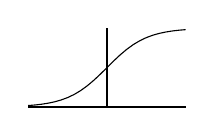
\begin{tikzpicture}[baseline={(0,0.2)}]
         \draw (-1,0) -- (1,0);
         \draw (0,0) -- (0,1);
         \draw plot[domain=-1:1,variable=\x] ({\x},{1/(1+exp(-4*\x))});
        \end{tikzpicture}\\
        \\
        tanh & $\sigma(x)=\frac{e^x-e^{-x}}{e^z+e^{-z}} $ & $\sigma'(x)=1-\sigma^2$   
        &  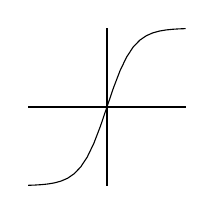
\begin{tikzpicture}[baseline={(0,0)}]
         \draw (-1,0) -- (1,0);
         \draw (0,-1) -- (0,1);
         \draw plot[domain=-1:1,variable=\x] ({\x},{tanh(3*\x)});
        \end{tikzpicture} \\
        ReLU & $\sigma(x) =\begin{cases}
        0 & ~\text{if}~ x<0 \\ 
        x & ~\text{if}~x \geq 0.
        \end{cases}$ & $\sigma'(x)=\begin{cases}
        0 & ~\text{if}~ x<0 \\ 
        1 & ~\text{if}~x > 0.
        \end{cases} $ & 
        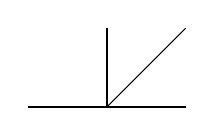
\begin{tikzpicture}[baseline={(0,0.5)}]
         \draw (-1,0) -- (1,0);
         \draw (0,0) -- (0,1);
         \draw plot[domain=-1:1,variable=\x] ({\x},{ifthenelse(\x<0,0,\x)});
        \end{tikzpicture}\\                      
    \end{tabular}
    \caption{Non-linear activation functions.}
    \label{tab:activationfct}
    \end{table}

\end{comment}

\section{Activation Functions}
There are many common activation functions with various strengths used in modern neural networks. We shall briefly mention a few ones
for completeness.

\subsection{Sigmoid and Tanh}
The sigmoid activation function is given by 
\begin{equation}\label{eq:sigmoid}
    \sigma(x) = \frac{1}{1 + \exp(-x)}.
\end{equation}
It was a very common choice in neural networks early, likely due to its simple derivative. It has a significant drawback, however.
Looking at eq.~\eqref{eq:sigmoid}, we can easily deduce that $\sigma(\pm \infty) = 0$, and since its derivative is of the form $\sigma'(x) = \sigma(1-\sigma)$,
the gradient computed during backpropagation vanishes if the input to the activation function as $\abs{x} \to \infty$. This significantly
hampers the progress during optimization. A popular alternative to the sigmoid function is $\tanh(x)$. This function is very similar to sigmoid in the sense that its derivative vanishes
for inputs of large magnitude and so may suffer from the same issues as sigmoid does.


\subsection{ReLU}
To overcome the vanishing gradient problem, an activation function called the Rectifying Linear Unit (ReLU) became widely adopted, which is given by
\begin{equation}
    \sigma(x) = x^+ = \max(0, x).
\end{equation}
% The activation was found to perform well in deep learning back in 2011 \cite{relu} and has become widely adopted.


\subsection{Swish}
Recently, an activation function to replace ReLU was proposed in \cite{swish} known as \textit{swish} or SiLU which was shown to outperform ReLU in deep neural networks on
a number of challengig datasets. The activation function is given by
\begin{equation}
    \sigma(x) = x\cdot \text{sigmoid}(x).
\end{equation}



\section{Bayesian learning of Neural Networks using Monte Carlo Samplers}
So far, we have discussed neural networks as a model class whilst ignoring the issue of what it really means to do Bayesian learning of neural networks, 
in other words, what it means to \textit{train} BNNs. We have intentionally left it somewhat ambigious what this really means because as it turns out, its meaning can be quite different depending on how Bayesian inference is performed. In this section we will clarify precisely what it means to train BNN using MCMC samplers such as HMC and NUTS. We shall then discuss practical aspects of the training which we shall put to practice in chapter \ref{chap:numerical_experiments}.

\subsection{What \textit{is} Bayesian learning of Neural Networks?}
The way Bayesian learning of neural networks manifest itself depends on the way in which we do Bayesian inference of the probabilistic model. 
We are concerned with inference of model parameters from the posterior using MCMC methods and will therefore obtain samples where each such sample
consist of the weights of an entire neural network. More precisely, if we gather $N$ samples with a chosen sampler, we will obtain $N$ entire neural networks
all sampled from the posterior to explain the observed data. Thus, what we mean by a \textit{trained} BNN in this sense is that we have
sampled a set of neural networks that collectively represent the BNN. 

As we discussed at the end of chapter \ref{chap:bayesian_ml}, 
we are mainly interested in the predictive distribution $p(y|x, W, b)$ of an output $y$ given an input $x$. We can approximate this distribution by constructing an empirical distribution by feeding $x$ through all $N$ sampled neural networks to obtain $N$ predicted targets $\hat{y}$ using eq.~\eqref{eq:predictive_dist_approx}.
The second quantity of interest is expectations of target functions dependent on the model parameters. 
We can approximate any such expectation with an MCMC estimator as in eq.~\eqref{eq:mcmc_estimator} using all $N$ networks to evaluate the target function.


\subsection{The Potential Energy Function of Neural Networks}

We now turn to the Bayesian formulation of the neural network model for use with the samplers used in this thesis. Assume that we have picked an architecture for a neural network and wish to train it in the Bayesian sense.
For both HMC and NUTS, we need only specify a potential energy function for our model. The samplers
take care of the rest. Assume we are dealing with a dataset $D = \{(x^{(i)}, y^{(i)})\}_{i=1}^N$ where all $N$ points are independent and identically distributed.
Equation~\eqref{eq:potential_energy_bayesian} instructs us to specify a prior for the weights of the network, and a likelihood function that depends on the target and the model output, in order
to fully specify the potential energy function.
Common practice is to choose priors that are either Gaussian or Laplacian. We will operate with Gaussian priors, i.e.
\begin{equation}\label{eq:model_priors}
  P(W^\ell) \propto \exp\left(-\frac{\lambda_W}{2}\norm{W^\ell}_2^2\right) \qq{and} \qquad P(b^\ell) \propto \exp\left(-\frac{\lambda_b}{2}\norm{b^\ell}_2^2\right).
\end{equation}
We will not worry too much about the choice of priors as the term in the potential energy function that corresponds to the likelihood will be much larger in practice. The Gaussian priors serve roughly the same purpose as $L^2$-regularization does in classical ML.

The likelihood for regression from eq.~\eqref{eq:likelihood_fn} formulated in terms of a neural network $\hat{f}(x^{(i)};W, b)$ is
\begin{equation}
  p(D|W, b) = \exp \left(-\frac{1}{2\sigma^2}\sum_{i=1}^N\norm{y^{(i)} - \hat{f}(x^{(i)};W, b)}_2^2\right).
\end{equation} 
This is not the only valid choice for a likelihood function but it is the common choice since it can be identified with the Euclidean $L^2$-norm and
itself ``neat'' mathematical properties.

Combining the priors and the likelihood with eq.~\eqref{eq:loss_function_of_posterior} yields the potential energy function
\begin{equation}\label{eq:special_potential_energy}
  \mathcal{L} = \frac{1}{2\sigma^2}\sum_{i=1}^N \norm{y^{(i)} - f(x^{(i)}; W, b)}_2^2 + \frac{\lambda_W}{2} \sum_{\ell=1}^L \norm{W^\ell}_2^2 + \frac{\lambda_b}{2}\sum_{\ell=1}^L \norm{b^\ell}_2^2,  
\end{equation}
up to a constant. As we discussed in chapter \ref{chap:hmc}, the potential energy function also happens to be the typical loss function with $L^2$-regularization used in the classical ML which is why we denote it as $\mathcal{L}$. At this point, we have set up all the machinery we need to train BNNs. Our next topic of discourse is the practice of doing so.

\subsection{Practical Training of Bayesian Neural Networks}

Training BNNs in practice requires us to specify a fairly large number of hyperparameters to obtain a set of models. These are 
\begin{enumerate}
  \item \textbf{Neural network architecture}. We need to specify its number of layers, number of nodes and activation function per layer. 
  Once the BNN is trained, we store this information along with the model for future usage. The stored weights themselves will encode how many layers and nodes the model has but the activation functions must be stored in addition.
  \item \textbf{Number of results}. We must specify how many neural networks we want to sample and store. Because the weights must be stored in its entirety, we are forced to worry about the amount of disk space that is required to do so. For a fixed allocated disk space, we can obviously store a larger set of samples if the model is simple. As complexity increases, the number of samples we can store will necessarily decrease.
  \item \textbf{Number of burn-in steps}. We must decide how long we want to run the MCMC chain before we start storing results. If amount of disk space was no obstacle, this step would be considered entirely optional as we could simply store every single sample and make a thorough analysis of the chain's quality to determine when proper mixing is obtained. In practice, with TensorFlow's framework, we can make a predetermined set of burn-in steps to avoid unnecessary RAM usage.
  \item \textbf{Amount of thinning}. Since successive samples most likely will be correlated, we can specify how many samples we simply skip once we start gathering samples, i.e. after the burn-in period. Again, we could ignore this and do this manually with the chain but doing so becomes a question of amount of available VRAM, RAM and disk space. 
  \item \textbf{Hyperparameters specific to the samplers}. The samplers themselves carry their own hyperparameters. In the case of HMC, we must specify a fixed number of Leapfrog steps $L$. If we use the NUTS sampler, we must specify the maximum tree depth. Moreover, we must determine how much of the computing resources we allocate to adapting the step size used in the Leapfrog integrator.
  \item \textbf{Amount of pretraining}. An attempt to accelerate convergence of the MCMC chain can be achieved by pretraining the neural network using minimization methods with the backpropagation algorithm to bring the weights closer to a minima of the potential energy function (i.e. the loss function used in classical ML). Then the point estimate obtained at the end of the training is used as a starting point for the MCMC chain.
\end{enumerate}

\subsection{Training Algorithm of Bayesian Neural Networks}
In this section we shall turn our attention to an actual training algorithm for BNNs. Assume we pick a sampler $S$ that represents either HMC or NUTS and a specified permuation of the hyperparameters discussed in the last section. In practice we can summarize a training algorithm as follows.
\begin{enumerate}
  \item Initialize the weights of the model from the specified priors, i.e.
  \begin{equation}
    W^\ell \sim p(W^\ell) \qq{and} b^\ell \sim p(b^\ell) \qq{for} \ell=1,\ldots, L.
  \end{equation}
  \item Minimize the potential energy function $\mathcal{L}$ with respect to the weights of the model using an optimizer of your choice to obtain a point estimate for use as the initial state of the Markov chain.
  \item Initialize the Markov chain for a finite set of burn-in steps to achieve mixing using $S$. A proportion of the initial burn-in steps are used for step size adaptation, while the remaining are used for mixing.
  \item Gather samples by applying $S$ repeatedly, replacing the current weights of the model by the ones returned by $S$.  
\end{enumerate}


\begin{comment}
  
With the ingredients discussed hitherto, it is time to consider practical training of BNNs.
We can divide this process in two parts. First, we must choose the architecture of the model, which is tantamount to picking model class. This decision is similar in nature to the training of regular neural networks to obtain point estimates. Second, we must consider the sampling process of the model. There are several considerations to make here such as disk space, length of mixing, amount of thinning and so on.

\subsection{Sampling of Bayesian Neural Networks}
We may divide this procedure into several subcategories:
\begin{enumerate}
  \item Choosing sampler $S$.
  \item Amount of mixing. We must choose the number of burn-in steps to run the sampling process before we actually start gathering sampled NNs.
  \item Amount of thinning. Number of samples to skip per stored sample. 
  \item Number of NNs to sample. Since the way we do Bayesian learning of NNs here actually require us a set of full NNs and store them to disk, we must decide how many samples we want to gather.
\end{enumerate}


\begin{enumerate}
  \item Initialize the weights of the network sampled from the priors. 
  \item An \textit{optional step}: train the network using a minimization algorithm with $\mathcal{L}$ as loss to reach an initial network state in the high probability \textit{density} region of the posterior.
  This is done to reduce the number of burn-in steps needed for the the Markov chain to reach the stationary distribution. However, for sufficiently high-dimensional parameter spaces this 
  may lead to adverse effects since the typical set may not be close to any mode of the posterior.
  \item Perform a finite number of burn-in steps to facilitate mixing by application of $S$ repeatedly.
  \item Sample a set of neural network parameters from the posterior distribution by use of $S$ repeatedly.
\end{enumerate}

\end{comment}

\chapter{Numerical Experiments}\label{chap:numerical_experiments}
\section{The Dataset}\label{sec:dataset}
In this section, we will describe the dataset and how it is generated. Moreover, we will discuss the data transformations prior to training and its implications on the accuracy of the predictions.
\subsection{Data Generation}


\subsection{Data Scaling and Transformations}
We shall briefly discuss how the training data is transformed before training.
The targets in the dataset of NLO cross sections can span several orders of magnitude. For practical training of BNNs, this would require
model parameters that also span several orders of magnitude. The result will usually be overflow and thus unsucessful training of the models.
Therefore, we have chosen to map the targets using the base-10 logarithm, i.e. $y \mapsto \log_{10}(y)$. More generally, we could choose any base-$a$ logarithm. A practical consideration here is that once the model is trained, any prediction it produces must be transformed back using
the inverse mapping. As we increase the value of $a$, the precision the model's prediction decreases. Thus a small error in log-space 
can result in a large error in what we may refer to as the target space, the larger the value of $a$ is. 

\subsection{Data Splitting}
The conventional way is to split the dataset $\mathcal{D}$ into three subsets: 
\begin{enumerate}
    \item A training set $\mathcal{D}_\text{train}$. This dataset usually contain the largest chunk of the dataset and is used to train the models.
    \item A validation set $\mathcal{D}_\text{val}$. This dataset is typically the smallest of the bunch and is sometimes used in classical machine learning problems to perform cross-validation or similar methods. The results measured here are typically used to select hyperparameters of the model.
    \item A test set $\mathcal{D}_\text{test}$. This partition is slightly larger than the validation set and is used as an out-of-sample check to measure the performance of a model. 
\end{enumerate}
We have selected to use a division of 80\% training data, 5\% validation data and 15\% as test data. In practice though, the notion of a validation set does not lend itself as easily to Bayesian ML tasks and we may in practice therefore use both the validation and test data as the test set.

\section{Methodology}
In this section, we shall explain the methodology used to train and test the BNNs explored in this thesis. We will explain the framework implementation, the selection of models and 

\subsection{Implementation}
We have utilized the Python libraries {\tt TensorFlow 2.7.0} and {\tt TensorFlow-Probability 0.15.0} to implement the BNNs. 
The implementation itself is available at \url{LEGG TIL URL HER}. Unfortunately, BNNs trained with HMC or NUTS has not been of interest for most of the deep learning community and as a result not particularly useful implementation of BNNs for these kind of samplers have been implemented directly into the either framework. Therefore, we created our own class that facilitates the usual kind of conveniences shipped with {\tt TensorFlow} such as the ability to automatically save, load or print the model architecture to screen. The class and its functionality is well-documented and made with the intention to be reused, expanded and modified. 

Both {\tt TensorFlow} and {\tt TensorFlow-Probability} handle execution on NVIDIA GPUs automatically with minimal effort on the user side, which we have utilized to generate our results. We will also provide measurements that indicate the expected speedup gained from using a GPU instead of a CPU for training of BNNs.
 

\subsection{Selection of Models and Hyperparameters}
In order to better understand the behaviour of BNNs, we have chosen to train a set of models whose details are listed in table \ref{tab:deep_models}. Each model consists of 1000 sampled neural networks. Each model is trained with $\tanh(x)$ as the activation function on the hidden layers, while the output layer uses an identity activation. We will refer this table whenever a model or a set of models selected from it is used. Otherwise, we will state the model architecture used and its hyperparameters explicitly. 
\begin{table}[h!]
    \centering
    \caption{
        The table shows the models used in this section. For each model, 1000 sampled networks were sampled to collectively represent each BNN model. We used 2500 warm-up steps (20\% burn-in and 80\% adaptation). We skipped 10 samples for each sampled network. We used 1000 pretraining epochs with a batch size of 32. The kernel used for each model was the NUTS kernel with a maximum of $L = 4096$ Leapfrog steps.
        The number of nodes per layer is shown in the ``Layers'' column.
        For each hidden layer, we used $\tanh(x)$ as the activation function. The final layer uses an identity function.
    }
\begin{tabular}{c@{\hspace{1cm}}c@{\hspace{1cm}} c}
\hline
      Model number & Layers & Number of parameters \\
\hline
    1 & 5-50-1 & 351\\
    2 & 5-50-50-1 & 2901\\
    3 & 5-50-50-50-1 & 5451\\
    4 & 5-50-50-50-50-1 & 8001\\
    5 & 5-50-50-50-50-50-1 & 10551\\
\hline
\end{tabular}
\label{tab:deep_models}
\end{table}


\subsection{Performance Metrics}\label{sec:perf_metrics}
In this section, we will discuss the performance metrics used to benchmark and measure the performance of the models trained in this thesis.
Due to the inherent probabilistic nature of the models trained, any output the model produces will be a distribution from which we can calculate
a sample mean and variance.

\subsubsection{Relative Error}
The first and simplest form of performance metric we can use is the \textit{relative error} which is defined as
\begin{equation}
    \epsilon(x^*) = \frac{y_\text{true}- \hat{y}_\text{mean}(x^*)}{y_\text{true}},
\end{equation}
where $y_\text{true}$ is the true target and $\hat{y}_\text{mean}(x^*)$ is the sample mean of the empirical predicitive distribution of the model.

\subsubsection{Standardized Residuals}
A particularly useful way to represent how well a probabilitic model performs is to study its \textit{standardized residual} which is given by
\begin{equation}
    z(x^*) = \frac{y_\text{true} - \hat{y}_\text{mean}(x^*)}{\hat{\sigma}(x^*)},
\end{equation}
where $\hat{\sigma}(x^*)$ is the square-root of the sample variance. The mathematical representation of the targets $y$ is that they can be decomposed as
\begin{equation}
    y = f(x) + \delta,
\end{equation}
for some true function $f(x)$ and a random noise $\delta \sim \mathcal{N}(0, 1)$, i.e it is distributed according to a standard Normal distribution. But in the case of data produced by \texttt{Prospino}, the noise is neglible which means that $y \approx f(x)$. The regression error obtained through the sample variance is therefore dominated by the predictive distribution computed by the model itself. In practice, we want a model whose distribution lies inside a Normal distribution for it to be considered a reliable model. This choice is somewhat arbitary of course as we could have opted for a model with a Gaussian distribution with a different variance and used that as a benchmarking measure instead. 



\section{Results}\label{sec:results}
\subsection{Computational Performance}

\subsubsection{CPU v. GPU Performance}
In figure \ref{fig:relative_performance}, we demonstrate the significant speedup that can be achieved
with GPU accelerated sampling when using {\tt TensorFlow-Probability} and its implementation of samplers. Here we have used HMC and a fixed $L = 512$ Leapfrog steps with XLA (Accelerated Linear Algebra) compilation enabled on the GPU. This is a highly optimized linear algebra execution engine that can significantly speed up code written with {\tt TensorFlow} run on the GPU \cite{xla}. The time measurements per sample was in the order of magnitude of seconds for the most complex models
tested. An important aspect for practical utilization of BNNs will be ease of training and accelerated sampling with NUTS or HMC, which is automatically achieved if the system can detect an NVIDIA GPU. Moreover, the full training time can be estimated by a few preliminary runs where execution time per sample is measured. This analysis is slightly more difficult when using NUTS. One can however set a maximum tree depth generated with {\tt BuildTree} which is also the case with the implementation employed by {\tt TensorFlow Probability}. As we argued in chapter \ref{chap:no_u_turn_sampler}, the additional computational cost added by NUTS per Leapfrog step is neglible given a sufficiently complex model and/or large dataset.
Thus one can simply perform the measurements using the implementation of HMC and estimate an upper-bound on the computational time defined by the setting of the maximum tree depth.

\begin{figure}
    \centering
    \includegraphics[scale=0.8]{figures/cpu_vs_gpu/cpu_vs_gpu_performance.pdf}
    \caption{The figure shows the relative measured execution time used per sample using $L = 512$ Leapfrog steps,
    as a function of number of parameters. The CPU measurements are done using an 8-core M1 CPU (Apple Silicon). The GPU measurements
    are made with an NVIDIA Tesla P100 GPU.
    }
    \label{fig:relative_performance}
\end{figure}

\subsubsection{Prediction Time}
As we discussed in the introduction, the execution time's order of magnitude when using {\tt Prospino} is in the order of hours. 
If BNNs are to serve as a viable alternative to these calculations, it must at least significantly reduce the time it takes to compute predictions. In figure \ref{fig:prediction_time}, we 
show the average execution time to compute predictions using all models in table~\ref{tab:deep_models}.
For each model, we randomly generated input points of correct dimension and computed predictions for up to 4096 input points simultaneously.
The execution times appear proportional to the number of input points provided for each model, which perhaps is not all that surprising. We can crudely infer by inspection that increasing the order of magnitude by one does the same for the execution time. Still, the order of magnitude for a single input point is at the order of a millisecond which is a significant speedup over {\tt Prospino} calculations. Both the sample mean of the predictions and the sample error is computed during the measurement. The measurements were performed on an M1 Apple Silicon CPU using {\tt perf\_counter} from the module {\tt time} provided by the standard library of Python.

The performance degradation that the computations in figure \ref{fig:prediction_time} suffers is inherently due to the limited vectorization capability of the CPU's computing units when performing matrix multiplications in the forward pass of the individual neural network models. The computation itself is performed with all 1000 sampled networks simultaneously, and so one might hypothesize that more specialized computing units may be able to handle several input points while applying all sampled networks at the same time. As it turns out, GPUs are excel at executing matrix multiplication and even more fortunate, {\tt TensorFlow} has added support for the built-in GPU on Apple Silicon system-on-chips. In figure \ref{fig:prediction_time_gpu} we can see the execution times achieved using the GPU to perform the same computations as before. In this case the order magnitude remains more or less the same in all the tests. Thus, computing predictions on several points can benefit greatly if the execution is employed on a GPU. Note, however, that the measured execution time of ``model 1'' is slightly slower than for more points which likely is due to the overhead introduced by using the GPU for such a simple model. Care must thus be taken when considering what type of hardware the computations should be performed with.

\begin{figure}
    \centering
    \includegraphics[scale=0.8]{figures/prediction_time/prediction_time.pdf}
    \caption{The figure shows the average prediction time to compute a prediction given a single input $x$ using the models in table \ref{tab:deep_models}. The average time used is measured in ms and is averaged over 1000 randomly sampled points. The measured time includes computation of the sample mean and sample error.
    }
    \label{fig:prediction_time}
\end{figure}

\begin{figure}
    \centering
    \includegraphics[scale=0.8]{figures/prediction_time/prediction_time_gpu.pdf}
    \caption{The figure shows the average prediction time using the built-in GPU on an M1 Apple Silicon system-on-chip to compute a prediction given a single input $x$ using the models in table \ref{tab:deep_models}. The average time used is measured in ms and is averaged over 1000 randomly sampled points. The measured time includes computation of the sample mean and sample error. 
    }
    \label{fig:prediction_time_gpu}
\end{figure}

\subsubsection{Loading Times}
Even if we have demonstrated a substantial speedup for predictions using BNNs, we have thus far ignored the fact that empirical distribution representing the weights of the BNN is stored on disk which typically means an solid state drive (SSD) with modern computing hardware. The memory bandwidth between the SSD and the faster forms of memory such as RAM, cache and registers becomes a potential bottleneck for performance. Although cache and registers introduce fast memory transfer of stored data to the computing units of the CPU, they typically boast a fairly limited capacity. Thus loading in the entire BNN model might not be viable and we may observe that once we need to models with a large number of parameters, the loading times dominate the computational cost involved with computing predictions. This added computional cost stems from the transfer of data back and forth between the RAM, and the cache and registers. An additional problem is that if the BNN model is simply used for a single prediction at a time, it might simply be loaded a single time before it is dumped from working memory all together. In this case, the initial load may dominate the computational cost all together. 

In figure \ref{fig:loading_times} we show the resulted loading times measured using an M1 Apple Silicon system-on-chip and {\tt time.perf\_counter} from Python. The memory allocated to the BNN models were deallocated manually using the {\tt del} operator provided by Python to ensure that each load of the model of the model was from the SSD. The models loaded in are the ones listed in table \ref{tab:deep_models}. Given the order of magnitude of the loading times displayed in the figure is approximately the same order of magnitude as the execution time, we have demonstrated that BNNs can provide a serious substitute for {\tt Prospino} calculations from a purely computational perspective. It remains to be seen if the predictions themselves are reliable enough for this substitution to be adopted, which we will explore in later sections.

\begin{figure}
    \centering
    \includegraphics[scale=0.8]{figures/computational_cost/loading_times.pdf}
    \caption{
        The figure shows the histograms of measured loading times in seconds using the models in table \ref{tab:deep_models}. The measurements were performed using {\tt time.perf\_counter} from Python using an M1 Apple Silicon system-on-chip. The time measurements consist of 1000 measurements for each model.
    }
    \label{fig:loading_times}
\end{figure}



\subsection{Posterior Distribution of Weights}
An important problem to consider is if we can even justify the use of Monte Carlo samplers to sample from the exact posterior instead of using the approximation employed by variational inference with a parameterized surrogate posterior which is the most ubiquitous method of training BNNs in the literature. The surrogate distribution is usually a factorized normal distribution of the form
\begin{equation}\label{eq:surrogate_dist}
    q \propto \prod_{i, j, \ell} \mathcal{N}(\mu_{ij}^\ell, (\sigma_{ij}^\ell)^2) \mathcal{N}(\mu_{j}^\ell, (\sigma_{j}^\ell)^2),
\end{equation}
meaning for each parameter in the model, we assume its posterior distribution can be written as an independent Gaussian distribution with a mean $\mu_{jk}^\ell$ and a standard deviation $\sigma_{ij}^\ell$ for the kernels, and $\mu_j^\ell$ and $\sigma_j^\ell$ for the biases. The method sports some fairly obvious advantages like the fact that one can perform \textit{online training}, i.e. continue training once new data becomes available starting from an earlier \textit{checkpoint} by using $q$ obtained during earlier training as the prior. The way we have trained BNNs in this thesis does not permit this form of training because we cannot formulate a prior based on the empirical distribution we have sampled. Thus we cannot use the weights of the model that we have already sampled to continue training. We must start over entirely and discard the empirical distribution we obtained with the prior dataset. 

It has been widely discussed that BNN posteriors are typically found to be multi-modal \cite{google_bnn_posteriors}. We demonstrate this observation in figure \ref{fig:posterior_kernels}.
We can observe that the projection onto the planes shown there indicate that the posterior distribution indeed is multimodal
and unlikely to be approximated well with a parameterized surrogate distribution like the one in eq.~\eqref{eq:surrogate_dist}.

\begin{figure}
    \centering
    \includegraphics[scale=0.7]{figures/posterior_distribution/posterior_weights1.pdf}
    \includegraphics[scale=0.7]{figures/posterior_distribution/posterior_weights2.pdf}
    \caption{The figure shows the projection of the empirical distribution onto the planes spanned by $(W_{2,4}^1, W_{2,5}^1)$ on the left and onto the plane spanned by $(W_{3,7}^1, W_{3, 6}^1)$ on the right, using the samples from model 3 in table \ref{tab:deep_models}. The distributions are approximated using kernel density estimation. 
    }
    \label{fig:posterior_kernels}
\end{figure}


\subsection{Benchmarks of Hyperparameters}\label{subsec:benchmarks}
\begin{figure}
    \centering
    \includegraphics[scale=0.7]{figures/computational_cost/time_vs_leapfrogsteps_hmc.pdf}
    \includegraphics[scale=0.7]{figures/computational_cost/time_vs_params.pdf}
    \caption{The figure at the top shows the measured time in seconds per sample using HMC as a function of Leapfrog steps $L$ using a model with
    561 parameters. The figure at the bottom shows the time in seconds per sample with the same sampler with a fixed number of Leapfrog steps $L = 512$ as a function of number of parameters in the BNN model.
    }
    \label{fig:time_vs_leapfrogsteps}
\end{figure}

\subsubsection{The Effect of Number of Burn-in Steps and Step Size Adaptation}
As we discussed in section \ref{sec:practical_bnn}, we must set a predetermined number of warm-up steps, i.e. number of burn-in steps and number of adaptation steps when using {\tt TensorFlow Probability}'s samplers.
Conventional wisdom would have us believe that increasing the number of burn-in steps increases the probability that the Markov chain has converged
to the stationary distribution of the posterior. Moreover, the literature has shown that NUTS performs at least as good as or better than HMC with an equivalent number of maximum Leapfrog steps or more as the results in \cite{nuts} demonstrated. In our case we have split the number of warm-up steps to 20\% burn-in steps and 80\% adaptation steps, respectively. This is a heuristic recommended by the {\tt TensorFlow Probability} developers.
In figure \ref{fig:standardized_residuals_vs_burn_in_steps} we demonstrate that the claims above may not be general enough to apply to BNNs as the HMC performs better almost regardless of how many burn-in/adaptation steps that are performed. When using NUTS, the performance of the model trained with a substantial amount of burn-in/adaptation steps appear to degrade as opposed to improve. The standardized residual of HMC lies consistently inside the Normal distribution for the most part, while the NUTS sampler produced few models that achieve the same. These results, then, actually indicate that we may be better off running the training procedure of BNNs with a fixed $L$, only adapting the step size. Even better, we may get by with a fairly limited amount of burn-in/adaptation steps and a fairly small $L$. The results in figure \ref{fig:standardized_residuals_vs_burn_in_steps} were generated with a fixed $L = 512$ Leapfrog steps when using the HMC sampler, while the NUTS sampler allowed for a maximum of $L = 4096$ Leapfrog steps. In figure \ref{fig:avg_leapfrog_steps_vs_burn_in}, we show the average number of Leapfrog steps the NUTS sampler used during the generation of the Markov chain as a function of number of warm-up steps.


\begin{figure}
    \centering
    \includegraphics[scale=0.7]{figures/standardized_residuals/effect_of_burnin/standardized_residuals_hmc_vs_burn_in_steps.pdf}
    \includegraphics[scale=0.7]{figures/standardized_residuals/effect_of_burnin/standardized_residuals_nuts_vs_burn_in_steps.pdf}
    \caption{The figure shows the standardized residuals computed on the testset. The model architechture used is a model with layers 5-20-20-1 with $\tanh(x)$ as the hidden activation function. In the top figure, we have used the HMC sampler with a fixed number of Leapfrog steps $L = 512$. In the bottom figure, we have used the NUTS sampler with a maximum tree depth of $12$ corresponding to a maximum of $L = 2^{12} = 4096$ Leapfrog steps. The remaining important hyperparameters were 2500 pretraining epochs with a batch size of 32 using the ADAM optimizer. In total a 1000 neural networks were sampled in each case with a thinning-amount of 10 steps between each sample.
    }
    \label{fig:standardized_residuals_vs_burn_in_steps}
\end{figure}


\begin{figure}
    \centering
    \includegraphics[scale=0.8]{figures/standardized_residuals/effect_of_burnin/avg_burnin_steps_nuts_vs_burn_in_steps.pdf}
    \caption{The figure shows the average number of Leapfrog steps $L$ as a function of number of warm-up steps used by the NUTS sampler when sampling the models shown in the bottom of figure \ref{fig:standardized_residuals_vs_burn_in_steps}. We have included a few more measurements to showcase how fluctuating the average number can be. 
    }
    \label{fig:avg_leapfrog_steps_vs_burn_in}
\end{figure}




\subsubsection{The Effect of Pretraining}
Pretraining a model before initiating the Markov chain is typically suggested as a means to accelerate convergence to the stationary distribution by minimizing a selected loss function with respect to the model parameters to obtain a point estimate. The point estimate is then used as the initial point of the Markov chain. This may help but as we discussed in chapter \ref{chap:mcmc}, the typical set, the set which we seek to sample from, may not lay particularly close to the mode of the loss function, or as we know it as, the potential energy function. Thus we have good reasons to challenge this recommendation and verify that it indeed improves the performance of the BNN models we sample. In figure \ref{fig:std_residual_vs_pretraining}, we
show the computed standardized residuals resulting from models trained with a varying amount of pretraining. Here all other
hyperparameters are fixed. The figure demonstrates a pretty noticable improvement as the amount of pretraining increases, up to a point. Once we surpass 2048 epochs of pretraining, we see a slight degradation of the model performance with a larger spread in the residual distribution. But we can rest assured that pretraining can be used to increase the performance of the trained BNN when everything else is held fixed. The various hyperparameters used are listed as part of the figure to avoid tedious repetition.


\begin{figure}
    \centering
    \includegraphics[scale=0.8]{figures/standardized_residuals/effect_of_pretraining/standardized_residuals_hmc_vs_pretraining_steps.pdf}
    \caption{The figure shows the standardized residuals of a model with the architecture 5-20-20-1 with $\tanh(x)$ as the
    hidden activation function. In this case the varying number of the number of epochs run with pretraining starting from 32 all the way up to 8192. The batch size used was 32, the number of warm-up steps was 1000 (200 of which were burn-in steps and 800 were adaptation steps). We fixed the Leapfrog steps to $L = 512$ using the HMC sampler. The ADAM optimizer was used for the pretraining phase. As usual we sampled 1000 neural networks with 10 steps between each sample.
    }
    \label{fig:std_residual_vs_pretraining}
\end{figure}

\subsubsection{Effect of Number of Parameters}
Increasing the number of parameters of the BNN model may help capture the underlying model from the data to a larger degree. The typical problems posed by the \textit{bias-variance trade-off} \cite{ml_for_physicists} (pages 12-13) does not play as significant a role here since the trained model can compute a sample variance along with its prediction. This does not mean it is immune, however, as the model will still sample according to the nuances found in the training data which in principle may be due to noise. As explained in section \ref{sec:perf_metrics}, the dataset produced by {\tt Prospino} contains very little noise and thus specializing the model to inherent noise is not the issue. Instead, we may be a bit unfortunate with the splitting of the dataset such that the training data itself contains information in some of its datapoints that are not present in the test data or vice versa. This may result in a model with a large set of parameters that produces poor results when generalizing to the unseen test data. Moreover, the dataset we use is fairly small (~ 16000 datapoints in total), which may exacerbate the overfitting effect.
In figure \ref{fig:standardized_residual_vs_params}, we show the computed standardized residual distribution of the models listed in table \ref{tab:deep_models}, which gives us an idea of the performance the BNNs have on this dataset as a function of the number of parameters. We can note that model 3 and 4 performs fairly well given our chosen benchmark measure, but that model 5's performance degrade somewhat, which is the model that contains the most parameters of the models tested. 

\begin{figure}
    \centering
    \includegraphics[scale=0.8]{figures/standardized_residuals/standardized_residual_simple_models.pdf}
    \caption{
        The figure shows the distribution of the standardized residuals computed on the test data using the models listed in table \ref{tab:deep_models}. The Normal distribution is drawn in with a dotted black line for benchmarking reference.
        The figure is meant to illustrate the performance of the models with respect to the number of parameters in the models.
        The models were trained with 2500 warm-up steps (20\% burn-in and 80\% adaptation), gathering 1000 neural networks with 10 steps between each sample. We used 1000 pretraining epochs with a batch size of 32. The kernel used was the NUTS kernel with a maximum of $L = 4096$ Leapfrog steps. 
    }
    \label{fig:standardized_residual_vs_params}
\end{figure}


\subsection{Neutralino-Neutralino Cross Sections}\label{subsec:neuralino_experiments}
\subsubsection{Predictive Distributions}
As we discussed in chapter \ref{chap:bayesian_ml}, one of the primary objects we seek to compute
in Bayesian ML is the predictive distribution $p(y^*|x^*, D)$ for a target $y^*$ given an unseen input point $x^*$ and
a training dataset $D$. In figure \ref{fig:predictive_distributions}, we show the predictive distribution computed with model 3 in table \ref{tab:deep_models}. In the figure on top, the sample mean approximates the true target well with a fairly small spread in the distribution which is a desirable outcome in most cases. There are, however, ill cases as well which we demonstrate in the figure at the bottom. Here the true target lies entirely outside the predictive distribution. Thus care must be taken to understand when a BNNs prediction is reliable and when it is not.
\begin{figure}
    \centering
    \includegraphics[scale=0.7]{figures/predictive_distributions/predictive_distribution_point_idx_360.pdf}
    \includegraphics[scale=0.7]{figures/predictive_distributions/predictive_distribution_point_idx_2052.pdf}
    \caption{
        The figure shows the predictive distribution estimated by use of model 3 in table \ref{tab:deep_models} for to randomly chosen points from the test set. The red line shows the true target and the black line shows the predicted sample mean obtained from the distribution. The figure on top demonstrates a case where the sample mean is approximately the same as the target, while the figure at the bottom demonstrates a case where the true target lies entirely outside the predictive distrbution. 
    }
    \label{fig:predictive_distributions}
\end{figure}



\begin{table}[h!]
    \centering
\begin{tabular}{c@{\hspace{1cm}}c@{\hspace{1cm}}c@{\hspace{1cm}}c@{\hspace{1cm}}c@{\hspace{1cm}}c}
\hline
    Burn-in steps & \makecell{Number \\of \\steps between} & Kernel & \makecell{Number \\ of \\ results} & \makecell{Pretraining \\ epochs} & \makecell{Pretraining \\ batch size} \\
\hline
    2500 & 10 & NUTS & 1000 & 1000 & 32 \\
\hline
\end{tabular}
\caption{
    The table shows the training configuration used to sample the models listed in table~\ref{tab:deep_models}.
}
\label{tab:NN_mse_scores}
\end{table}





%\input{Sections/QFT/Axiomatic}
%\input{Sections/QFT/Pertubationtheory}
%\input{Sections/QFT/StandardModel}
%%%%%%%%%%%%%%%%%%%%%%%%%%%%%%%%%%%%%%%%%%%%%%%%%%%%%%%%%%%
%\input{Sections/QFT/MathematicalFormulationGaugeTheories}
%\input{Sections/QFT/WilsonGeometry}

%%%%%%%%%%%%% Wilson Line Properties %%%%%%%%%%%%%%%%%%%%%%%%
%\chapter{Wilson Line Properties}
%\input{Sections/WilsonLineProperties/CuspAnomalous}

%\chapter{Supersymmetry}
%\input{Sections/SUSY/Supersymmetry}

%%%%%%%%%%%%% QCD %%%%%%%%%%%%%%%%%%%%%%%%
% \chapter{Perturbative Quantum Chromodynamics}\label{Chap:pQCD}
% \input{Sections/QCD/LagrangianQCD}
% \input{Sections/QCD/DIS}
% \input{Sections/QCD/DrellYan}



%%%%%%%%%%%%% Conclusion %%%%%%%%%%%%%%%%%%%%%%%%%%
\chapter*{Conclusion}\label{chap:conclusion}
% \newpage
% \chapter*{Conclusion}
% \addcontentsline{toc}{chapter}{Conclusion}
The main objective of this thesis has been to investigate Bayesian neural networks sampled from the exact posterior as a substitute for direct calculations of next-to-leading order cross sections in quantum field theory. We argued for the necessity of bypassing the computationally expensive direct calculations with Bayesian regression because of the need for an estimate of the uncertainty of the predicted cross sections. This was due to the role the uncertainties play in the statistical exclusion of regions in parameter spaces of possible Beyond the Standard Model theories. The neural network model was chosen for its universal function approximation property. We provided an overview of Bayesian machine learning and its relation to classical machine learning with a focus on regression tasks. We sought to use Markov chain Monte Carlo methods to sample from the exact posterior of neural networks and thus delved into the theory behind these methods for continuous sample spaces, building our way through the Metropolis-Hastings methods all the way up to the advanced class of samplers used in this thesis, namely Hamiltonian Monte Carlo. We discussed the shortcomings of Hamiltonian Monte Carlo with a fixed trajectory length and its need for tedious hand-tuning via preliminary diagnostic tests. This motivated the exploration of adaptive Hamiltonian Monte Carlo techniques to adapt the trajectory length with the No-U-Turn sampler for the number of Leapfrog steps and a dual-averaging scheme for the step size used in the Leapfrog integration component. 

Through numerical experiments, we demonstrated that trained BNNs can significantly reduce the time spent computing cross sections. We found that the time spent on such computations were roughly evenly divided between loading the models in from memory and performing the actual forward pass in the neural networks to compute the predictive distribution, its sample mean and sample variance. Moreover, we found that the training employed on GPUs with XLA compilation can result in a significant reduction in training time compared to training on CPUs.
We investigated the empirical posterior distribution of the sampled weights and found them to be multi-modal, consistent with claims in the literature, sowing doubt of the reliability of Bayesian inference using surrogate models. We explored how various hyperparameters used during training of BNNs affect their predictive performance. We found evidence suggesting that a moderate amount of warm-up steps and pretraining positively impacts the performance of the trained models but that an excessive amount exacerbated it. With the vast set of different configurations one can use with BNNs though, these results may not be generalizable to different forms of architectures than the ones we have used and more extensive investigations can be carried out. Some of the configurations we explored were found to produce reliable uncertainty estimates and performed well in the space of targets it was trained for. Finally, we explored the predictive distributions of a trained BNN model and showcased an example of a good predictive distribution and a predictive distribution which missed the mark entirely. We showed that the BNN model underperformed relative to a Normal distribution where less than 96 \% of the targets resided within $\pm 2\sigma$ of the sample mean of the distributions. 

Although we have progressed our understanding of the training of BNNs by drawing samples from the exact posterior with MCMC samplers like HMC and NUTS, there are several question which we have not answered. We propose the following problems to be addressed in the future.
\begin{enumerate}
    \item \textbf{The Convergence Properties of the Markov Chain}. In chapter \ref{chap:mcmc}, we noted that the standard metric to estimate that a Markov chain has converged to its stationary distribution were by use of the scale reduction factor $\hat{R}$. Such convergence statistics is not measured or reported in this thesis. Computing $\hat{R}$ for neural network posteriors is complicated by the non-identifiability of neural networks. Several different neural networks sampled from the different regions of sample space may produce the same predictions, which makes assessing the convergence by studying the elements of the Markov chain itself challenging. Instead we propose the use of $\hat{R}$ computed on the predictions by using the samples in the Markov chain. This analysis has been performed in \cite{google_bnn_posteriors} where they study the resulting Markov chain in function space. For a specific input $x$, one can run several independent chains that all compute their own predictive distribution. The $\hat{R}$ metric can then be calculated from the resulting set of distributions to identify potential non-convergence.
    \item \textbf{Training of BNNs on Larger Datasets}. In this thesis, we have focused on a fairly small dataset of $\sim 15000$ datapoints. At no point have we investigated the added computational expense from computing the potential energy function and its gradient in HMC and NUTS as a function of the number of datapoints it needs to be evaluated for. If NLO cross section estimation is to be used with BNNs on larger datasets, the effect it has on the hyperparameters used during training is likely necessary to be reinvestigated. The analysis performed in this thesis should at least give information on what hyperparameters that are worth exploring. Training time will likely be much longer but the predictive performance of the trained BNN may become more robust.
    \item \textbf{Sampling Larger Models}. Our analysis has been dealing with a fairly small number of sampled neural networks per model. In each case, we have drawn 1000 neural networks which collectively represented the full BNN model. The number of parameters the models had, spanned from a few hundred to the order of a hundred thousand. A thousand samples drawn from the posterior is a pretty low number owed to the computational expense needed to generate them. For the most complex models trained, the training time could exceed 24 hours on a GPU. Thus drawing more samples by running longer Markov chains can be exceedingly expensive. The potential upside is that the MCMC estimators and the predictive distributions will likely produce better results if more samples are drawn. An important consideration to reduce the training time is to increase the complexity of neural networks by adding many small layers and create deep networks as opposed to shallow networks with many nodes per layer. The reason for this is that applying shallow ``wide'' networks to a large dataset simultaneously during training may create temporary objects which are too large to fit into cache and registers which results in additional time spent transferring strips of memory, in which case the GPU may sit idle during large portions of the training.
    \item \textbf{The Effect of Thinning}. We have operated with a fixed number of samples skipped between each drawn network. This means that we have performed no analysis of the correlation between successively drawn samples but instead worked with a heuristic that appeared to produce good results. Investigating the \textit{lag}-$l$ autocorrelation of successive neural network samples can give valuable information from a practical perspective. Although drawing more samples may be beneficial for the calculation of MCMC estimators, it is not so if the samples are heavily correlated. Both samplers used in this thesis generate successive samples with low correlation in simple cases studied in the literature \cite{nuts,neal2011} but with the complexity of the BNN posterior, this may require a larger amount of thinning. Performing preliminary runs to estimate how correlated successive samples are will help reduce the necessary amount of samples needed to be drawn to obtain good statistics from the MCMC estimators. It will also help the practitioner to minimize the amount of thinning and avoid wasting computational resources.
    \item \textbf{The Effect of the Multi-modality of the Posterior on the Predictive Distributions}. Although we demonstrated the multi-modality of the posterior distribution of BNNs, we did not investigate its effect on the predictive distribution. After all, it is the predictive distribution we really care about in practice. Due to how computationally expensive it is to sample from the exact posterior, a thorough comparison of sampling from the exact posterior should be compared and contrasted with the use of surrogate distributions for the BNNs parameters with respect to the quality of the predictive distributions they produce.
    \item \textbf{Other Potential Energy Functions}. In our investigation we have used a Gaussian prior for each neural network parameter and the same likelihood function for each model. It is possible that modifying the potential energy function, either by choosing different priors or modifying the likelihood function, that the training process can be improved. It has been suggested that the effect of the chosen priors may yield a measurable impact on the predictive distribution although it may not be particularly noticable from studing the posterior distribution of weights \cite{google_bnn_posteriors}.
    \item \textbf{Deep Ensembles}. Deep ensembles has been shown to yield a better fidelity of the Bayesian predictive distribution on par with the ones produced by HMC, outperforming the surrogate distributions typically employed in the literature \cite{google_bnn_posteriors}. And this can potentially be achieved at a significant reduction of the computational cost of sampling from the true posterior using HMC or NUTS. 
    \item \textbf{Multi-GPU Training with HMC}. In this thesis, within the framework we used, we were confined to run the sampling on a single GPU device. Investigating the possibility of running multiple independent Markov chains on several GPUs simultaneously in an asynchronous fashion can potentially speed up the training of BNNs with HMC significantly by allowing for many long chains to sample independently of each other. The quality of the sampled chains from the posterior is likely to improve by generating more than a single chain. One possible framework to adopt for this is Jax \cite{jax}, a machine learning research library developed and used in-house by the Deep Mind research team at Google Research. It allows for automatic mapping of a Python function to several physical devices (such as multiple GPUs), just-in-time compilation for GPU devices which when run on NVIDIA GPUs support XLA compilation. Moreover, it provides its own framework for automatic differentiation. Thus it may be a viable platform to develop more research oriented machine learning models than the more strict frameworks provided by TensorFlow and its extensions. Due to the complex control flow introduced by the NUTS sampler, it is not as well suited for multi-GPU sampling but other adaptive schemes such as ChEES-HMC was recently proposed to adaptively set the trajectory length without the same limitation \cite{chees-hmc}.
    \item \textbf{Approximate the Prior From the Empirical Distribution for Online Training}. A major drawback to drawing samples from the exact distribution is that we in practice must discard old models when new data becomes available. This is unfortunate as we obviously know \textit{something} about the weights inferred from the dataset prior to the arrival of the hypothetical new data. We are closely guarding a set of them which we have drawn, informed by the ``old'' data. In order to increase the viability of sampling from the exact posterior, investigating ways to obtain approximate unnormalized densities that approximate the empirical distributions can be fruitful for the following reason. The potential energy function used in HMC and NUTS \textit{requires} the ability to evaluate a log prior given an arbitrary input of weights. Thus inferring a function that approximates the empirical distribution will yield an \textit{informed} prior that can be evaluated to draw new samples given new data. This can greatly increase the viability of the methods as old samples can inform the generation of new ones. 
\end{enumerate}
\backmatter{}
%%%%%%%%%%%%% Appendix %%%%%%%%%%%%%%%%%%%%%%%%

\begin{appendices}
\numberwithin{equation}{section}

\appendix
\chapter{Appendix A}
\renewcommand{\thechapter}{A}
\renewcommand{\theequation}{\thechapter.\arabic{equation}}
\section{Appendix 1 title }\label{sec:appendix_1_label}
Some appendix stuff.



% \appendix
% \renewcommand{\thechapter}{B}
% \chapter{Appendix B}
% \input{Sections/Appendix/Appendix2}
%
% \appendix
% \renewcommand{\thechapter}{C}
% \chapter{Appendix C}
% \renewcommand{\theequation}{\thechapter.\arabic{equation}}
% \input{Sections/Appendix/Appendix3}
%
% \appendix
% \renewcommand{\thechapter}{D}
% \chapter{Appendix D}
% \renewcommand{\theequation}{\thechapter.\arabic{equation}}
% \input{Sections/Appendix/Appendix4}


\end{appendices}




\bibliography{bibliography.bib}

\end{document}
